% Springer Nature manuscript draft for Paper 2: full-data sewing-pattern reconstruction experiment.

\documentclass[pdflatex,sn-mathphys-num]{sn-jnl}

\usepackage{graphicx}
\usepackage{amsmath,amssymb,amsfonts}
\usepackage{booktabs}
\usepackage{array}
\usepackage{url}
\usepackage{xcolor}
\usepackage[section]{placeins}

\raggedbottom
\setlength{\textfloatsep}{8pt plus 1pt minus 2pt}
\setlength{\floatsep}{8pt plus 1pt minus 2pt}
\setlength{\intextsep}{8pt plus 1pt minus 2pt}
\renewcommand{\bibfont}{\footnotesize}

\begin{document}

\title[Full-Data Pattern Reconstruction Benchmark]{A Full-Data Sewing-Pattern Reconstruction Benchmark for 3D Garment Modeling: Evidence Audit, Mesh Quality, Pattern Structure, and Retrieval Baselines}

% Author and affiliation metadata are omitted for double-anonymous review.

\abstract{Pattern-aware 3D garment modeling requires evidence beyond surface meshes, including editable panels, stitch relations, segmentation, renders, and specifications. This paper reports a full-data benchmark on the Dataset of 3D Garments with Sewing Patterns. We checksum-verified all 14 Zenodo files, totaling 84.77 GB, and audited 22,457 samples directly from compressed archives. The 22,450-sample production subset spans 12 garment categories. Beyond file completeness, we parse simulated and scan-imitation meshes, extract pattern-graph descriptors, define a pattern-mesh consistency score, and evaluate retrieval-style reconstruction baselines on a deterministic 70/15/15 split. Overall, 22,452 of 22,457 samples are complete, yielding a 99.98\% complete-evidence rate; 22,448 production samples achieve perfect pattern-mesh consistency. Pattern complexity ranges from 2 to 9 panels and from 4 to 18 stitches, while mean simulated mesh complexity ranges from 11,992 to 37,743 faces. Mesh-only retrieval reaches 77.32\% top-1 accuracy, segmentation reaches 88.12\%, deterministic render descriptors reach 99.73\%, and combined structured features reach 99.97\%. Hard-generalization tests show that the random split is mainly an in-distribution benchmark: leave-one-category-out render descriptors retain 52.92\% mean family transfer but only 13.14\% panel-exact transfer, and descriptor noise reduces render top-1 retrieval to roughly 12--13\%. The benchmark provides a reproducible basis for image-to-pattern retrieval, pattern-structure prediction, and later traditional-garment extensions.}

\keywords{3D garment modeling, sewing pattern reconstruction, garment dataset, pattern graph, retrieval baseline}

\maketitle

\section{Introduction}\label{sec:intro}

Three-dimensional garment modeling has moved from surface-only clothing geometry toward structured garment representations. For tasks such as virtual try-on, digital fashion, avatar dressing, simulation, and cultural garment preservation, a plausible rendered surface is not enough. A research-ready garment asset should expose editable two-dimensional panels, seam or stitch relations, body-relative placement, segmentation, metadata, and simulation-ready three-dimensional geometry. Without those linked forms of evidence, a generated garment may look plausible while remaining impossible to edit, sew, simulate, or evaluate as a construction-aware digital object. This distinction is especially important when garment modeling is used not only for visual synthesis, but also for pattern reconstruction, parametric design, and later transfer to garments whose construction details carry cultural meaning.

This requirement is visible in recent literature. The Dataset of 3D Garments with Sewing Patterns provides generated garments with paired three-dimensional and sewing-pattern evidence \cite{korosteleva2021dataset}. GarmentCode and GarmentCodeData formalize garments as programmable parametric sewing patterns \cite{garmentcode2023,garmentcodedata2024}. NeuralTailor, Neural Sewing Machines, Panelformer, and SewFormer target pattern reconstruction or structure-preserving garment modeling from images, point clouds, or partial garment observations \cite{neuraltailor2022,nsm2022,panelformer2024,sewformer2023}. DrapeNet studies garment generation and self-supervised draping, showing the continuing importance of geometry and simulation-aware evaluation \cite{drapenet2023}. More recent systems such as Design2GarmentCode and GarmentDiffusion further connect garment design, program synthesis, and generative pattern creation \cite{design2garmentcode2025,garmentdiffusion2025}. Together, these methods show that the bottleneck is not only model design; it is also the availability, completeness, and reliability of paired pattern-mesh-render evidence at scale.

The research gap is that many pattern-reconstruction papers evaluate models or introduce representations without first reporting whether the underlying corpus is complete enough for reproducible full-data experiments. Subset demonstrations can hide missing files, inconsistent segmentation, degenerate meshes, incomplete pattern specifications, or category templates that make retrieval easier than genuine reconstruction. Image-only garment datasets are valuable for geometry or appearance, but they do not necessarily expose editable panels and stitch relations. Conversely, structured garment datasets can support stronger reconstruction studies only if their pattern, mesh, render, segmentation, and specification evidence are jointly verified. A benchmark therefore needs to measure not only how many samples exist, but also whether those samples can support controlled splits, interpretable baselines, and hard generalization protocols.

The present study focuses on that data layer. Before training or evaluating a pattern-reconstruction model, we ask whether a full downloadable structured garment corpus contains enough complete, consistent, and diverse evidence to support such experiments. We also ask which modalities make reconstruction-style retrieval easy, which modalities remain ambiguous, and whether high random-split retrieval accuracy survives harder tests such as leave-one-category-out transfer, paired template transfer, and descriptor perturbation. The study is deliberately full-data rather than subset-based: all files in the Zenodo record are downloaded, checksum-verified, and audited. The motivation includes future traditional-garment modeling, such as Vietnamese \textit{ao dai} pattern generation, but the immediate contribution is a reproducible benchmark of an existing structured garment dataset.

This emphasis on benchmark construction is practical rather than merely administrative. A learned reconstruction model can appear strong if the train and test samples share a narrow set of templates, colors, or rendering conventions, even when the method has not learned transferable garment construction. A full-data audit can reveal this by separating evidence completeness from reconstruction difficulty and by comparing weak-input settings against upper-bound pattern-assisted settings. It also gives future researchers a stable reference point: if a new model claims improvement, the improvement can be compared against transparent retrieval baselines, per-category diagnostics, and hard splits rather than against a loosely described subset.

The novelty of the work is not a new neural architecture. Instead, it is a full-data measurement protocol that links evidence completeness, mesh quality, pattern-graph structure, segmentation consistency, retrieval baselines, render baselines, and hard-generalization analysis in one manuscript. This framing is useful because it separates three questions that are often conflated: whether the data exist, whether the data are internally consistent, and whether simple baselines already solve the in-distribution task. The resulting benchmark can serve as a pre-training gate for learned methods, a sanity check for future image-to-pattern papers, and a template for extending structured garment reconstruction toward culturally specific garments. It also makes the limitations explicit: controlled synthetic renders can be easy for deterministic descriptors, while held-template or real-photo reconstruction remains a different and harder claim.

The contributions are:
\begin{itemize}
\item a full-data download and checksum-verification protocol for the 84.77 GB Zenodo sewing-pattern garment corpus;
\item an archive-level audit of 22,457 garment samples without requiring full extraction to disk;
\item category-level measurements of evidence completeness, panel count, stitch count, SVG pattern count, mesh quality, and segmentation consistency;
\item a pattern-mesh consistency score linking 2D pattern structure, 3D mesh evidence, and segmentation labels;
\item stratified train-validation-test splits and retrieval-style reconstruction baselines using pattern, mesh, segmentation, and combined feature sets;
\item hard-generalization protocols that test leave-one-category-out transfer, paired template transfer, and render-descriptor noise sensitivity;
\item publication-ready visual evidence showing representative render-pattern pairs across 12 production categories;
\item an experimental foundation for later image-to-pattern retrieval, pattern-structure prediction, parametric garment-program generation, and traditional-garment data collection.
\end{itemize}

\section{Methods}\label{sec:methods}

\subsection{Dataset, Evidence, and Audit Protocol}

\subsubsection{Dataset and Scope}

The experiment uses the public Dataset of 3D Garments with Sewing Patterns \cite{korosteleva2021dataset}. The Zenodo record contains 14 files: 13 zip archives and one datasheet PDF. All files were downloaded using resumable transfer and verified against the MD5 checksums provided by the Zenodo API. The verified compressed corpus size is 84,768,495,305 bytes. Two archives had already been used in a prior experiment and were reused through verified hardlinks; all remaining archives were downloaded and verified in the same pipeline.

The audit covers 22,457 samples. Of these, 22,450 belong to 12 production garment categories and 7 belong to the official \texttt{test.zip} archive. Production categories include pants, skirts, sleeveless tees, tees, sleeveless dresses, waistband dresses, waistband pants, jumpsuits, jackets, and hooded jackets. The official test samples are retained in the full audit count but excluded from category-comparison interpretation unless explicitly stated.

\subsubsection{Evidence Model}

Each garment sample is represented as
\begin{equation}
G_i = (I_i, P_i, S_i, M_i, A_i),
\end{equation}
where $I_i$ denotes rendered visual evidence, $P_i$ denotes 2D sewing-pattern evidence, $S_i$ denotes stitch or seam structure, $M_i$ denotes 3D mesh evidence, and $A_i$ denotes JSON specification attributes. The required evidence set is
\begin{equation}
E = \{I_f,I_b,P_{png},P_{svg},M_{sim},M_{scan},S_{sim},S_{scan},A\}.
\end{equation}
Here $I_f$ and $I_b$ are front and back renders, $P_{png}$ and $P_{svg}$ are raster and vector pattern files, $M_{sim}$ and $M_{scan}$ are simulated and scan-imitation OBJ meshes, $S_{sim}$ and $S_{scan}$ are segmentation files, and $A$ is the sample specification.

For sample $i$, the evidence-completeness score is computed as
\begin{equation}
C_i=\frac{100}{|E|}\sum_{e\in E}\mathbb{1}(e\in G_i).
\end{equation}
The audit further extracts panel count, pattern-edge count, stitch count, SVG path count, simulated mesh vertices and faces, and scan-imitation mesh vertices and faces.

\subsubsection{Archive-Level Audit}

The audit reads samples directly inside compressed archives. This design avoids expanding the full 84.77 GB compressed corpus into a much larger working directory and makes the experiment easier to resume. For each archive, the pipeline enumerates sample folders, checks required evidence entries, parses the garment specification, counts vector pattern elements, and scans mesh files for vertex and face records. The output records one structured measurement row per sample and a separate category-level summary, enabling both full-corpus statistics and per-category diagnostics.

\subsubsection{Visual Evidence Generation}

Two manuscript figures are generated from the full audit outputs. The first selects four representative complete samples per production category using mesh-complexity quantiles and composes render-pattern evidence from the verified archive images. The second summarizes mean simulated mesh complexity together with mean panel and stitch counts for each production category. Both figures are generated from the same verified data used by the quantitative benchmark.

\subsection{Metrics and Consistency}

\subsubsection{Mesh Quality and Pattern-Graph Metrics}

For the production subset, a second full pass parses both simulated and scan-imitation OBJ meshes. For each mesh, the benchmark computes vertices, faces, used and unused vertices, unique edges, boundary edges, non-manifold edges, connected components, duplicate vertices, degenerate faces, mean and median edge length, 95th-percentile edge length, mean and median triangle area, mean aspect ratio, and 95th-percentile aspect ratio. A triangle with side lengths $(a,b,c)$ is assigned aspect ratio
\begin{equation}
R_\Delta=\frac{\max(a,b,c)}{\max(\min(a,b,c),\epsilon)} ,
\end{equation}
where $\epsilon=10^{-12}$ prevents division by zero for degenerate triangles.

The sewing specification is parsed as a pattern graph. Panels are nodes and stitch rules define edges between panels. For each garment, the benchmark computes panel count, pattern-edge count, stitch count, graph components, panel areas, panel perimeters, curved-edge count, and parameter count. Segmentation files are parsed line by line to compute segmentation label counts, panel-label counts, stitch-label fraction, and label entropy.

\subsubsection{Pattern-Mesh Consistency Score}

The benchmark defines a learning-free pattern-mesh consistency score to summarize whether the available evidence is jointly usable for reconstruction experiments. For sample $i$, the score averages ten binary or fractional checks:
\begin{equation}
Q_i=100\cdot\frac{1}{10}\sum_{k=1}^{10} q_{ik}.
\end{equation}
The checks verify the presence of pattern panels, stitch rules, simulated mesh, scan-imitation mesh, zero non-manifold edges for each mesh, sufficient segmentation panel labels relative to pattern panels, and agreement between segmentation-line counts and mesh-vertex counts for both mesh types. Segmentation label coverage is fractional when fewer panel labels than pattern panels are observed:
\begin{equation}
q_{\mathrm{seg}}=\min\left(1,\frac{L_{\mathrm{panel}}}{\max(P,1)}\right),
\end{equation}
where $L_{\mathrm{panel}}$ is the number of non-stitch segmentation labels and $P$ is the number of pattern panels.

\subsection{Baselines and Generalization Protocols}

\subsubsection{Retrieval and Reconstruction Baselines}

To move from data audit to benchmark evaluation, the production subset is split by category into 70\% training, 15\% validation, and 15\% test samples. The test split contains 3,368 samples and the training split contains 15,715 samples. We evaluate nearest-neighbor retrieval baselines using four feature groups: pattern features, mesh features, segmentation features, and combined features. Continuous features are standardized using training-set statistics. For each test sample $x$, the nearest training samples are ranked by squared Euclidean distance,
\begin{equation}
d(x,z)=\|\hat{x}-\hat{z}\|_2^2.
\end{equation}
The retrieved neighbor is also treated as a simple reconstruction baseline for predicting panel and stitch counts. The evaluation reports top-1 accuracy, top-5 accuracy, mean reciprocal rank (MRR), panel-count mean absolute error, and stitch-count mean absolute error.

\subsubsection{Render-Image Retrieval Baseline}

Because many reconstruction settings begin from rendered or photographed garments rather than meshes or segmentation labels, we also evaluate a deterministic render-to-pattern retrieval baseline. For each production sample, front and back renders are read directly from the verified archives. Each view is converted into a 375-dimensional descriptor consisting of a \(16\times16\) grayscale thumbnail, edge-filter responses, 16-bin RGB histograms, channel means, channel standard deviations, and a view-presence indicator. The paired render descriptor concatenates front-view features, back-view features, and the absolute front-back feature difference:
\begin{equation}
\phi_I(G_i)=\left[\phi_f(G_i),\phi_b(G_i),|\phi_f(G_i)-\phi_b(G_i)|\right].
\end{equation}
Nearest-neighbor retrieval is evaluated on the same 70/15/15 split as the structured-feature baselines. Missing renders are represented by zero descriptors with the presence indicator set to zero, preserving the full 22,450-sample production scope.

\subsubsection{Hard-Generalization Protocols}

The stratified split measures in-distribution retrieval, but it can overstate reconstruction generalization when category identity and sewing-pattern templates are tightly coupled. We therefore add three harder protocols. First, leave-one-category-out evaluation trains the nearest-neighbor index on 11 categories and tests on the excluded category. Because the exact category is absent from the training set, the evaluation reports family-level transfer, exact panel-count transfer, exact stitch-count transfer, and panel/stitch mean absolute error rather than ordinary category top-1 accuracy. Second, paired transfer trains on one related source category and tests on a target variant, such as straight-side pants to waistband pants or jacket to hooded jacket. Third, render-noise stress keeps the original split but adds Gaussian perturbations to the test render descriptors. These protocols are intended to diagnose benchmark difficulty, not to replace task-specific learned reconstruction models.

\begin{table}[!htbp]
\caption{Algorithmic summary of the implemented full-data benchmark.}\label{tab:algorithm}
\centering
\footnotesize
\begin{tabular}{ll}
\toprule
Step & Operation \\
\midrule
1 & Input archives $\mathcal{Z}$ and checksum manifest $\mathcal{H}$ \\
2 & Verify $\mathrm{MD5}(z)=\mathcal{H}(z)$ for all $z\in\mathcal{Z}$ \\
3 & For each sample $G_i$: parse renders, pattern files, specs, segmentations, meshes \\
4 & Compute $C_i=100|E_i|/|E|$ and missing-evidence indicators \\
5 & Compute pattern graph descriptors $\phi_P(G_i)$ \\
6 & Compute mesh descriptors $\phi_M(G_i)$ for simulated and scan meshes \\
7 & Compute segmentation descriptors $\phi_S(G_i)$ \\
8 & Compute consistency score $Q_i$ from $\phi_P,\phi_M,\phi_S$ \\
9 & Build stratified splits $\mathcal{D}_{tr},\mathcal{D}_{val},\mathcal{D}_{te}$ \\
10 & Evaluate nearest-neighbor baselines using $\phi_P$, $\phi_M$, $\phi_S$, and concatenated features \\
\bottomrule
\end{tabular}
\end{table}

\begin{figure}[!htbp]
\centering
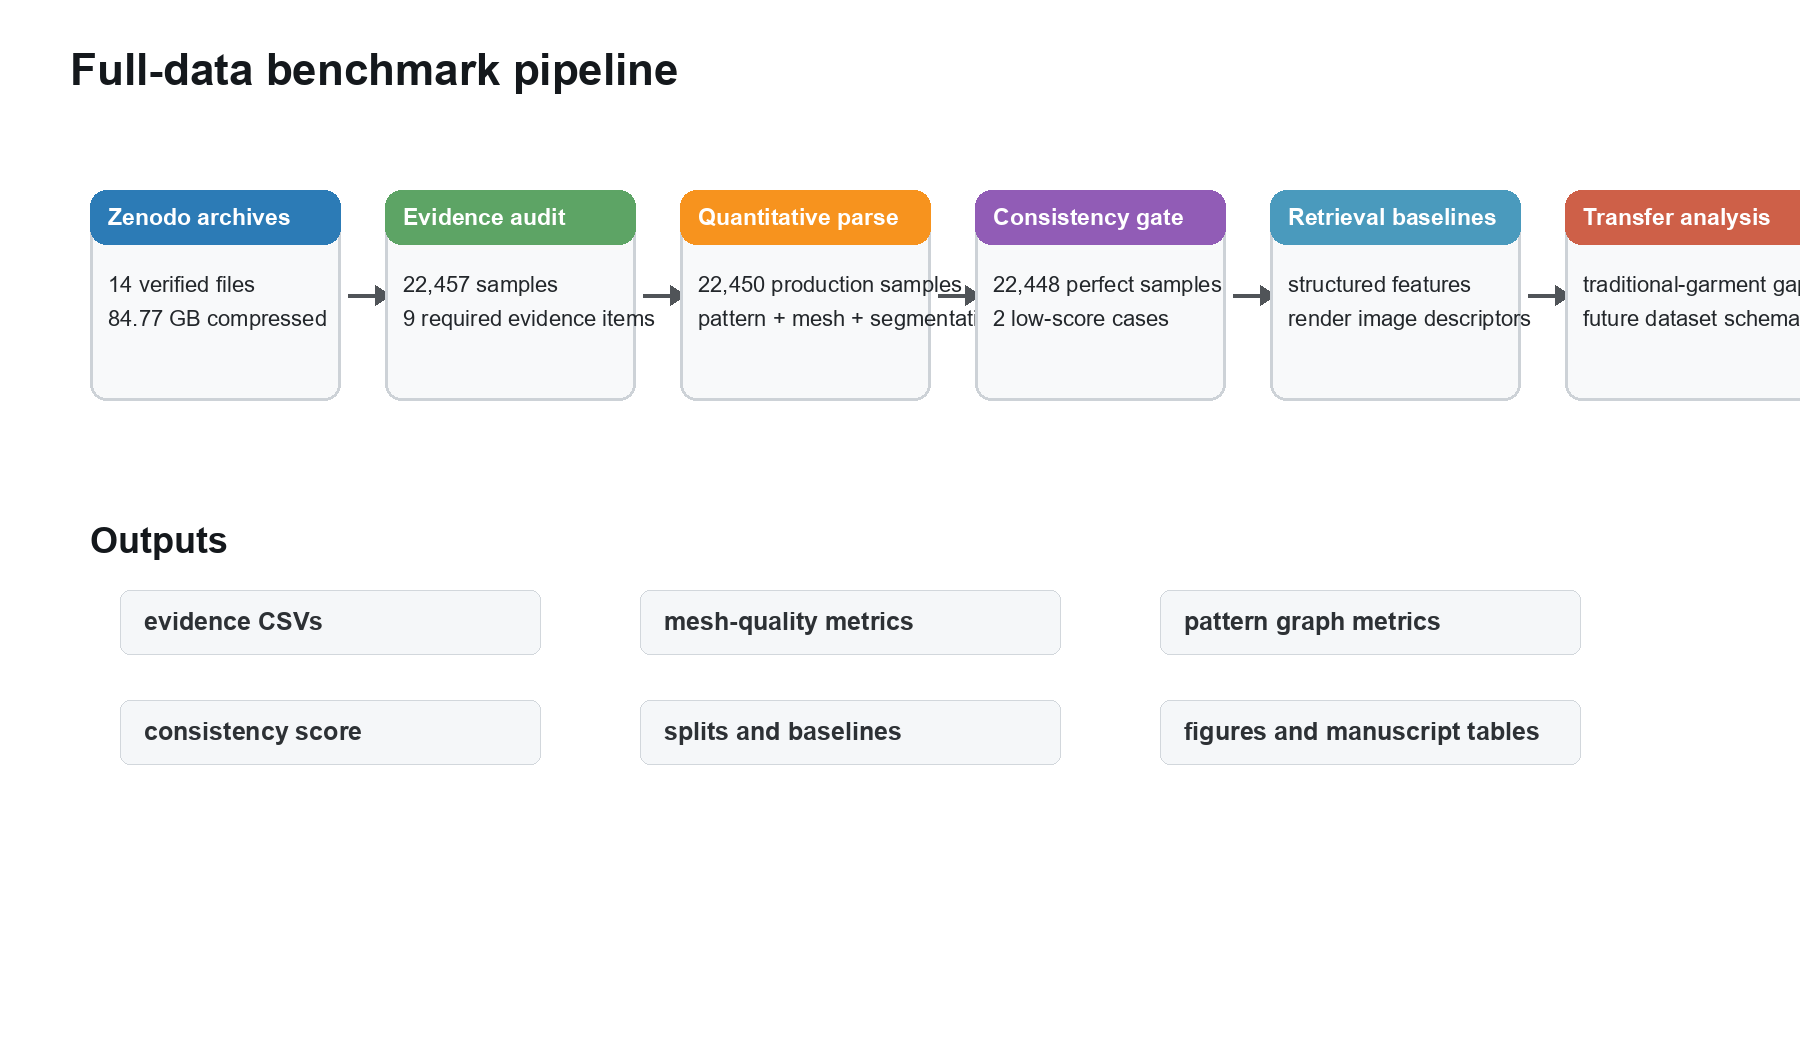
\includegraphics[width=\textwidth]{figures/fig_benchmark_pipeline.png}
\caption{Overview of the full-data benchmark pipeline and its main outputs. Each stage is implemented as a reproducible script and writes inspectable CSV, JSON, markdown, or figure artifacts.}
\label{fig:pipeline}
\end{figure}

\section{Results}\label{sec:results}

\subsection{Evidence and Category Structure}

\subsubsection{Full Download and Verification}

All 14 files in the Zenodo record were verified successfully. The verified corpus includes 84.77 GB of compressed data. The final audit contains 22,457 samples: 22,450 production samples and 7 official test samples. The full experiment completed with 22,452 complete samples, corresponding to a complete-evidence rate of 99.98\%. Only five samples have missing evidence.

\begin{table}[!htbp]
\caption{Full-data scope and evidence completeness.}\label{tab:scope}
\centering
\footnotesize
\begin{tabular}{lr}
\toprule
Measurement & Value \\
\midrule
Verified Zenodo files & 14/14 \\
Verified compressed bytes & 84,768,495,305 \\
Production categories & 12 \\
Production samples & 22,450 \\
Official test samples & 7 \\
Total audited samples & 22,457 \\
Complete samples & 22,452 \\
Samples with missing evidence & 5 \\
Complete-evidence rate & 99.98\% \\
\bottomrule
\end{tabular}
\end{table}

\subsubsection{Category Coverage and Pattern Complexity}

Table~\ref{tab:categorysummary} reports the full production category summary. The dataset spans low-complexity garments such as straight-side pants and two-panel skirts, intermediate garments such as dresses and jumpsuits, and high-complexity garments such as jackets and hooded jackets. Pattern complexity ranges from two panels and four stitches in simple skirts or sleeveless tees to nine panels and eighteen stitches in hooded jackets. Mean simulated mesh complexity ranges from 11,992 faces for straight-side pants to 37,743 faces for hooded jackets.

\begin{table}[!htbp]
\caption{Production category summary from the full 22,450-sample garment-pattern audit. \(C\) is mean evidence completeness. \(F_s\) is mean simulated face count. P/E/S gives mean panel, pattern-edge, and stitch counts.}\label{tab:categorysummary}
\centering
\footnotesize
\setlength{\tabcolsep}{3pt}
\begin{tabular*}{\textwidth}{@{\extracolsep{\fill}}lrrrrr}
\toprule
Category & \(N\) & Complete & \(C\) & \(F_s\) & P/E/S \\
\midrule
Pants straight sides & 1,000 & 1,000 & 100.000 & 11,992 & 4/20/6 \\
Skirt 2 panels & 1,200 & 1,200 & 100.000 & 12,908 & 2/12/4 \\
Skirt 4 panels & 1,600 & 1,600 & 100.000 & 15,140 & 4/24/8 \\
Jumpsuit sleeveless & 2,000 & 1,999 & 99.967 & 16,682 & 6/39/14 \\
Dress sleeveless & 2,550 & 2,547 & 99.965 & 17,894 & 4/29/10 \\
Skirt 8 panels & 1,000 & 999 & 99.989 & 22,669 & 8/48/16 \\
Tee sleeveless & 1,800 & 1,800 & 100.000 & 25,737 & 2/17/4 \\
WB pants straight & 1,500 & 1,500 & 100.000 & 26,036 & 6/30/12 \\
Jacket & 2,200 & 2,200 & 100.000 & 35,060 & 7/36/12 \\
Tee & 2,300 & 2,300 & 100.000 & 35,166 & 6/33/12 \\
WB dress sleeveless & 2,600 & 2,600 & 100.000 & 36,784 & 6/33/12 \\
Jacket hood & 2,700 & 2,700 & 100.000 & 37,743 & 9/47/18 \\
\bottomrule
\end{tabular*}
\end{table}

\begin{figure}[!htbp]
\centering
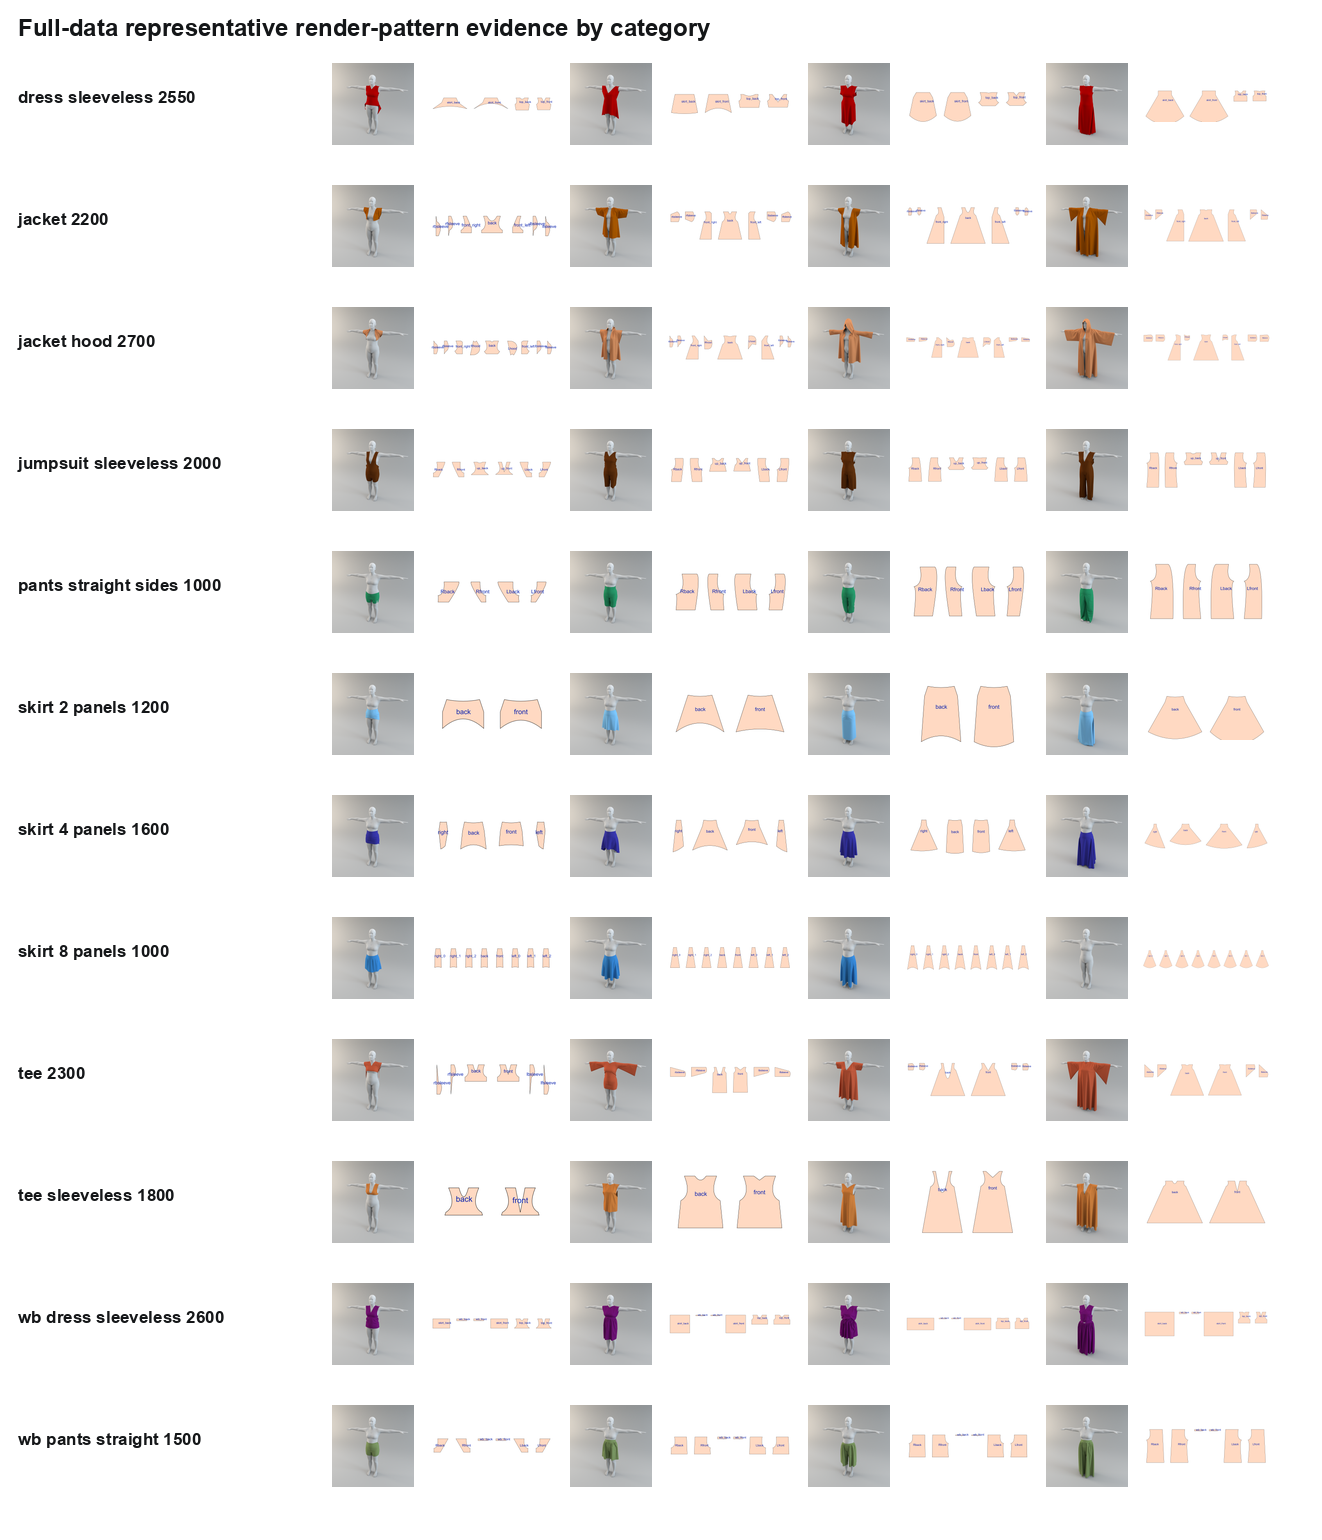
\includegraphics[width=\textwidth,height=0.86\textheight,keepaspectratio]{figures/fig_full_category_render_pattern_evidence.png}
\caption{Full-data representative render-pattern evidence by production category. For each category, four complete samples are selected by simulated mesh-complexity quantiles and shown as paired rendered garment views and sewing-pattern images.}
\label{fig:evidence}
\end{figure}

\begin{figure}[!htbp]
\centering
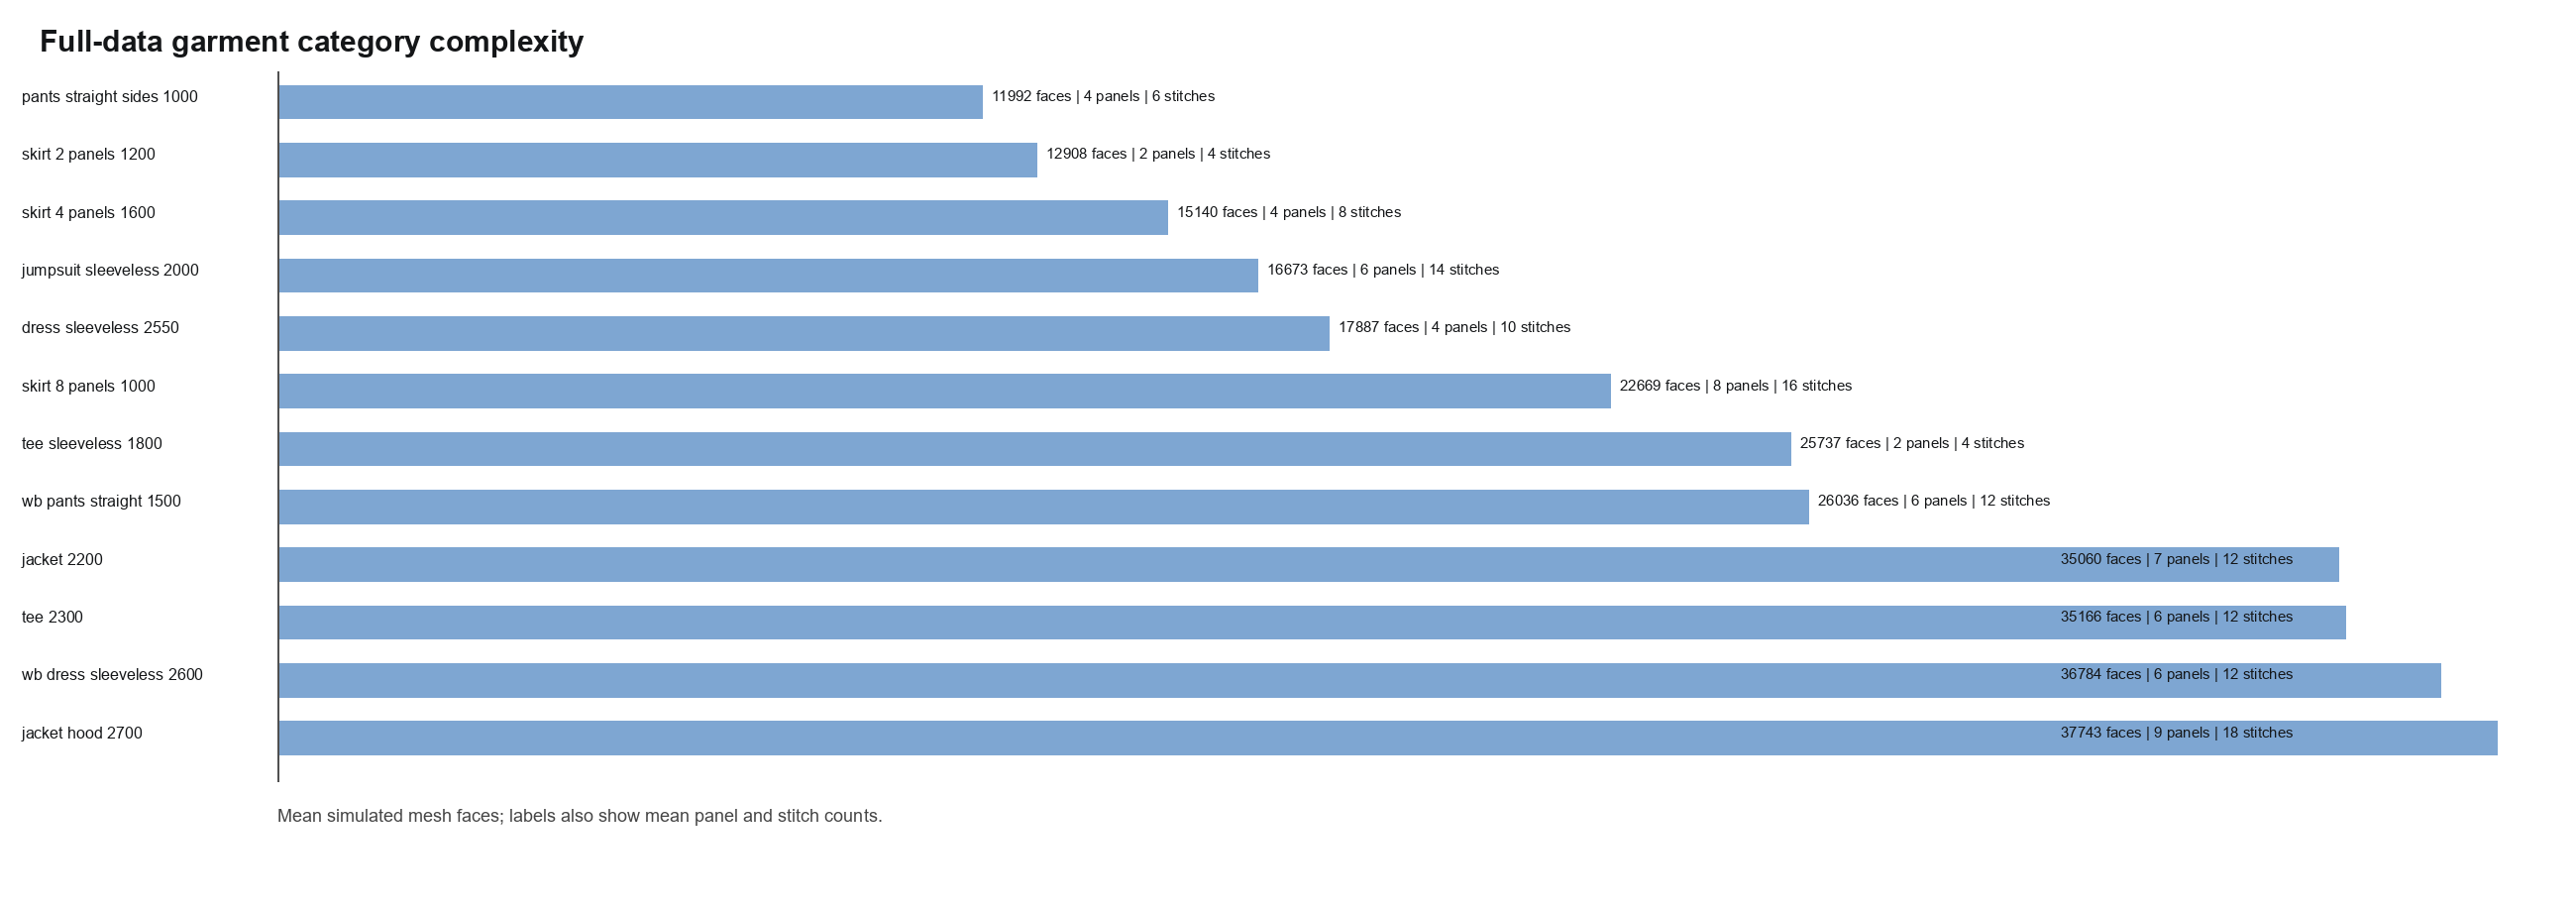
\includegraphics[width=\textwidth,height=0.50\textheight,keepaspectratio]{figures/fig_full_category_complexity_chart.png}
\caption{Full-data category complexity summary. Bars show mean simulated mesh faces; text labels report the corresponding mean panel and stitch counts.}
\label{fig:complexity}
\end{figure}

\subsubsection{Missing Evidence}

Missing evidence is rare. The five incomplete samples occur in three production categories: sleeveless dresses, sleeveless jumpsuits, and eight-panel skirts. Missing items include five missing front renders, two missing back renders, two missing simulated OBJ meshes, two missing scan-imitation OBJ meshes, and corresponding segmentation files. This suggests that the full dataset is highly usable for pattern-reconstruction experiments, although split construction should either exclude the five incomplete samples or explicitly mark them as failure cases.

\subsection{Mesh, Pattern, and Consistency Results}

\subsubsection{Mesh Quality Benchmark}

The quantitative benchmark parses 22,450 production samples and computes mesh descriptors for both simulated and scan-imitation meshes. Table~\ref{tab:meshquality} shows that mean simulated face counts range from 11,992 for straight-side pants to 37,743 for hooded jackets. Scan-imitation meshes are usually slightly lighter than simulated meshes, with the largest reductions appearing in skirt-8 and waistband-dress categories. Across categories, mean triangle aspect ratios remain close to 1.33--1.35, indicating mostly regular triangulation under the implemented metric. Non-manifold edges are zero at category mean level, while boundary edges remain nonzero because garment surfaces are open along hems, seams, and garment boundaries.

\begin{table}[!htbp]
\caption{Full production mesh-quality summary from simulated and scan-imitation meshes. AR denotes mean triangle aspect ratio.}\label{tab:meshquality}
\centering
\footnotesize
\setlength{\tabcolsep}{3pt}
\begin{tabular*}{\textwidth}{@{\extracolsep{\fill}}lrrrrrrr}
\toprule
Category & \(N\) & Sim faces & Scan faces & Sim boundary & Scan boundary & Sim AR & Scan AR \\
\midrule
Pants straight sides & 1,000 & 11,992 & 11,134 & 147 & 341 & 1.341 & 1.342 \\
Skirt 2 panels & 1,200 & 12,908 & 12,542 & 204 & 293 & 1.348 & 1.349 \\
Skirt 4 panels & 1,600 & 15,140 & 13,854 & 259 & 612 & 1.342 & 1.342 \\
Jumpsuit sleeveless & 2,000 & 16,673 & 16,072 & 222 & 569 & 1.338 & 1.338 \\
Dress sleeveless & 2,550 & 17,887 & 17,309 & 278 & 471 & 1.341 & 1.341 \\
Skirt 8 panels & 1,000 & 22,669 & 17,814 & 351 & 1,511 & 1.334 & 1.338 \\
Tee sleeveless & 1,800 & 25,737 & 24,786 & 369 & 642 & 1.336 & 1.336 \\
WB pants straight & 1,500 & 26,036 & 23,860 & 191 & 813 & 1.334 & 1.334 \\
Jacket & 2,200 & 35,060 & 33,955 & 544 & 1,123 & 1.334 & 1.334 \\
Tee & 2,300 & 35,166 & 34,051 & 399 & 733 & 1.335 & 1.335 \\
WB dress sleeveless & 2,600 & 36,784 & 32,812 & 337 & 1,148 & 1.335 & 1.337 \\
Jacket hood & 2,700 & 37,743 & 35,685 & 548 & 1,083 & 1.335 & 1.335 \\
\bottomrule
\end{tabular*}
\end{table}

\begin{figure}[!htbp]
\centering
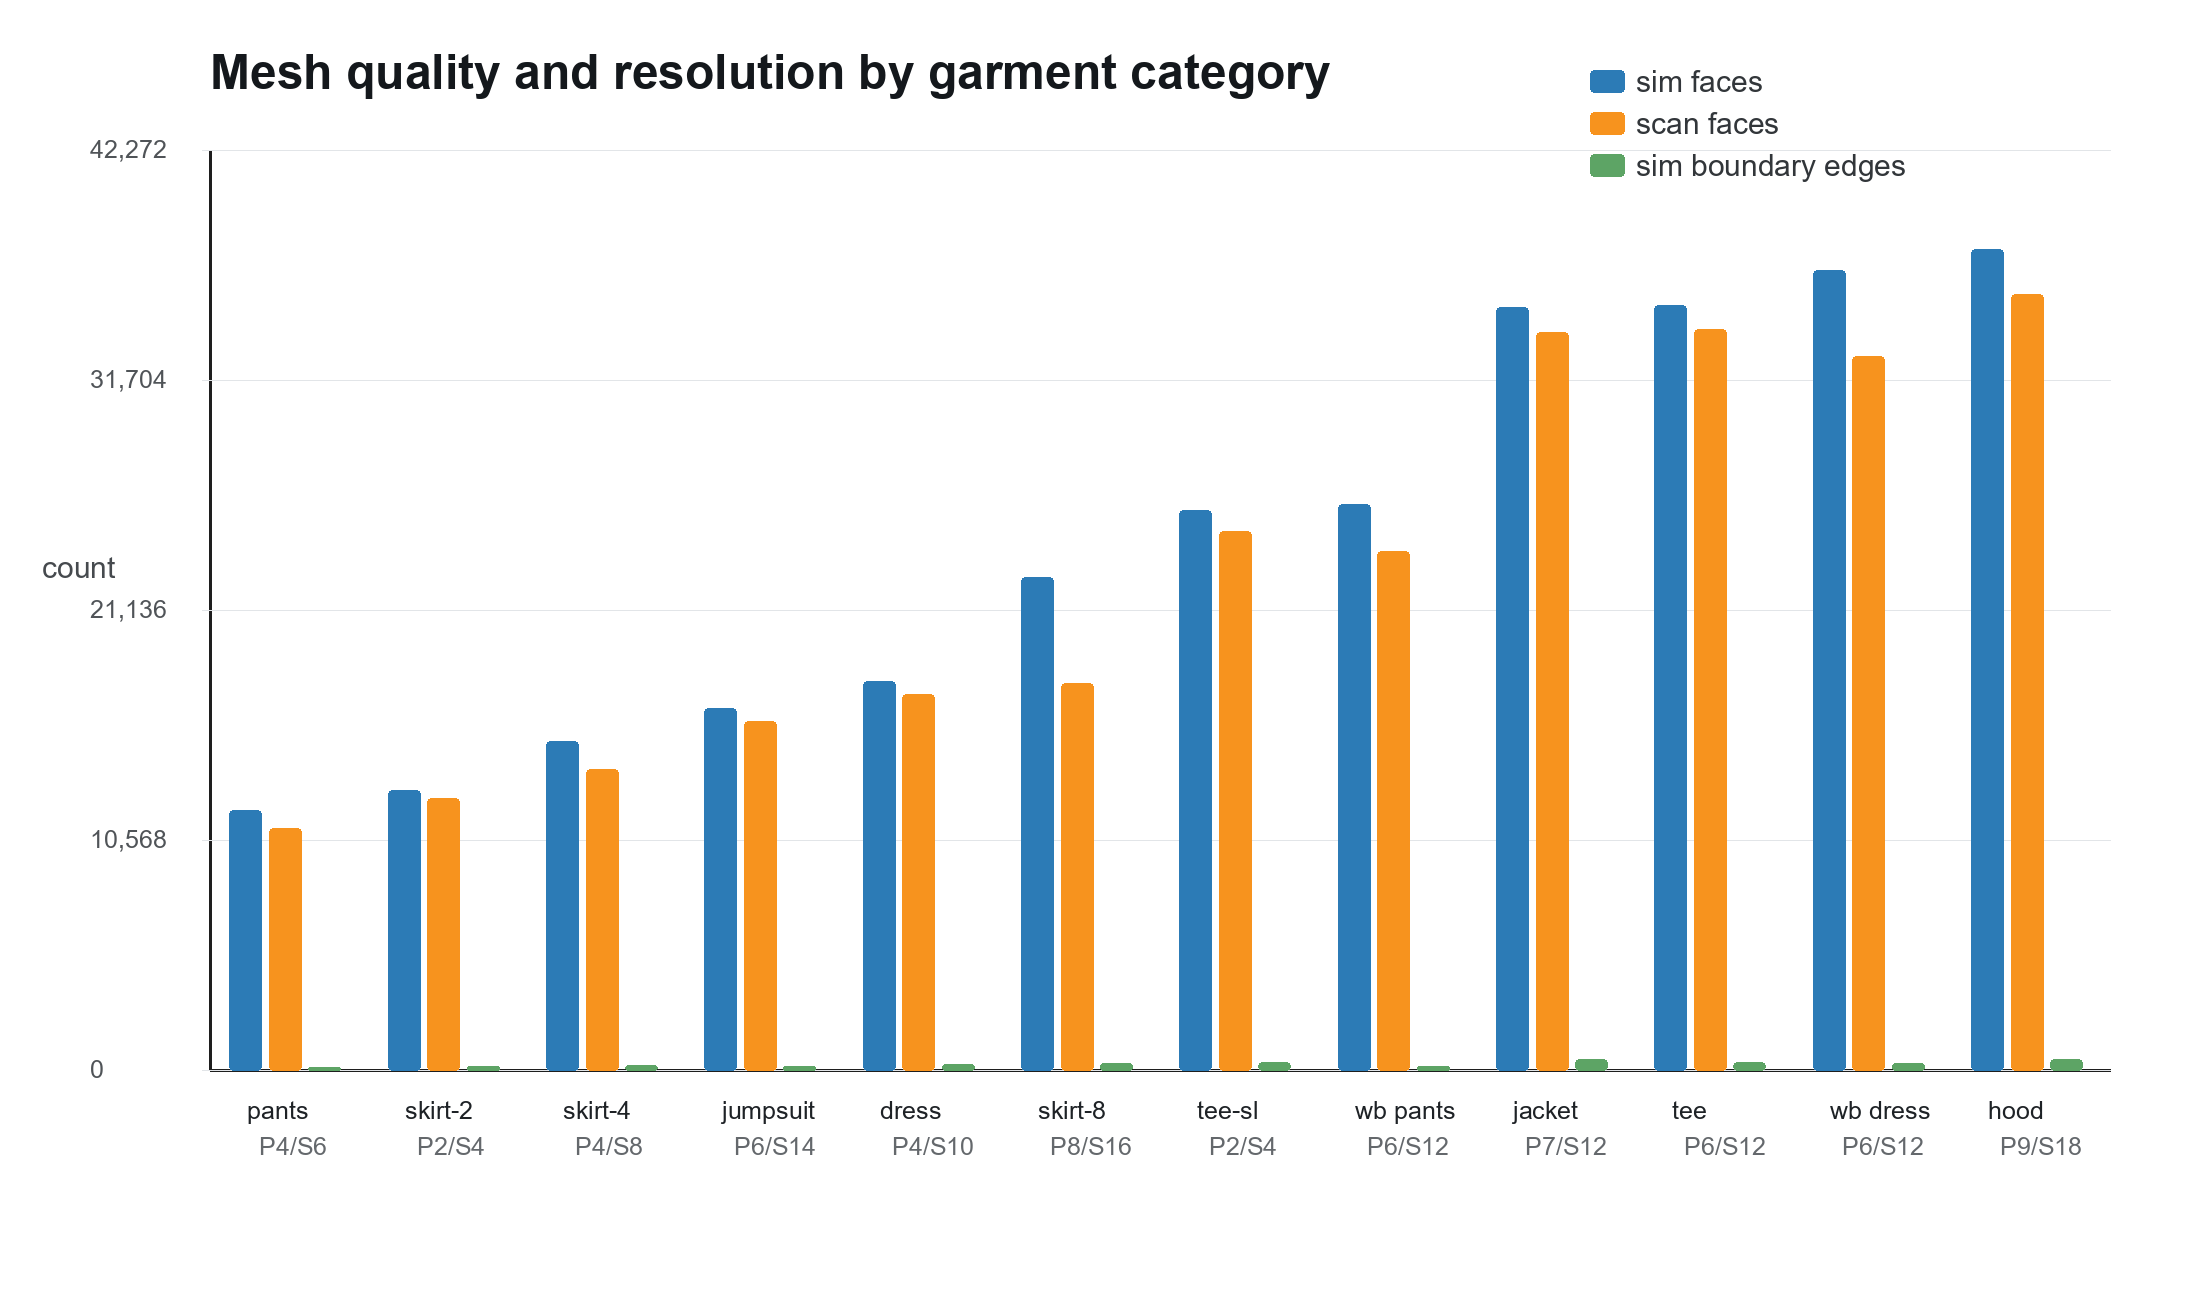
\includegraphics[width=\textwidth]{figures/fig_mesh_quality_by_category.png}
\caption{Mesh-quality and resolution summary by garment category. Simulated and scan-imitation face counts provide a category-level difficulty signal; boundary edges are included as a geometric openness indicator.}
\label{fig:meshquality}
\end{figure}

\subsubsection{Pattern Structure Benchmark}

The pattern-graph benchmark confirms that the corpus contains a structured complexity ladder rather than a flat set of templates. Simple categories such as two-panel skirts and sleeveless tees contain two panels and four stitches. Intermediate categories include pants with four panels and six stitches, sleeveless dresses with four panels and ten stitches, and jumpsuits with six panels and fourteen stitches. The most complex category, hooded jackets, contains nine panels and eighteen stitches. Figure~\ref{fig:patternstructure} visualizes the category-level panel, stitch, and curved-edge statistics. Figure~\ref{fig:skirtladder} isolates the skirt categories, showing that panel count, stitch count, boundary edges, and mesh resolution increase together from two-panel to eight-panel skirts.

\begin{figure}[!htbp]
\centering
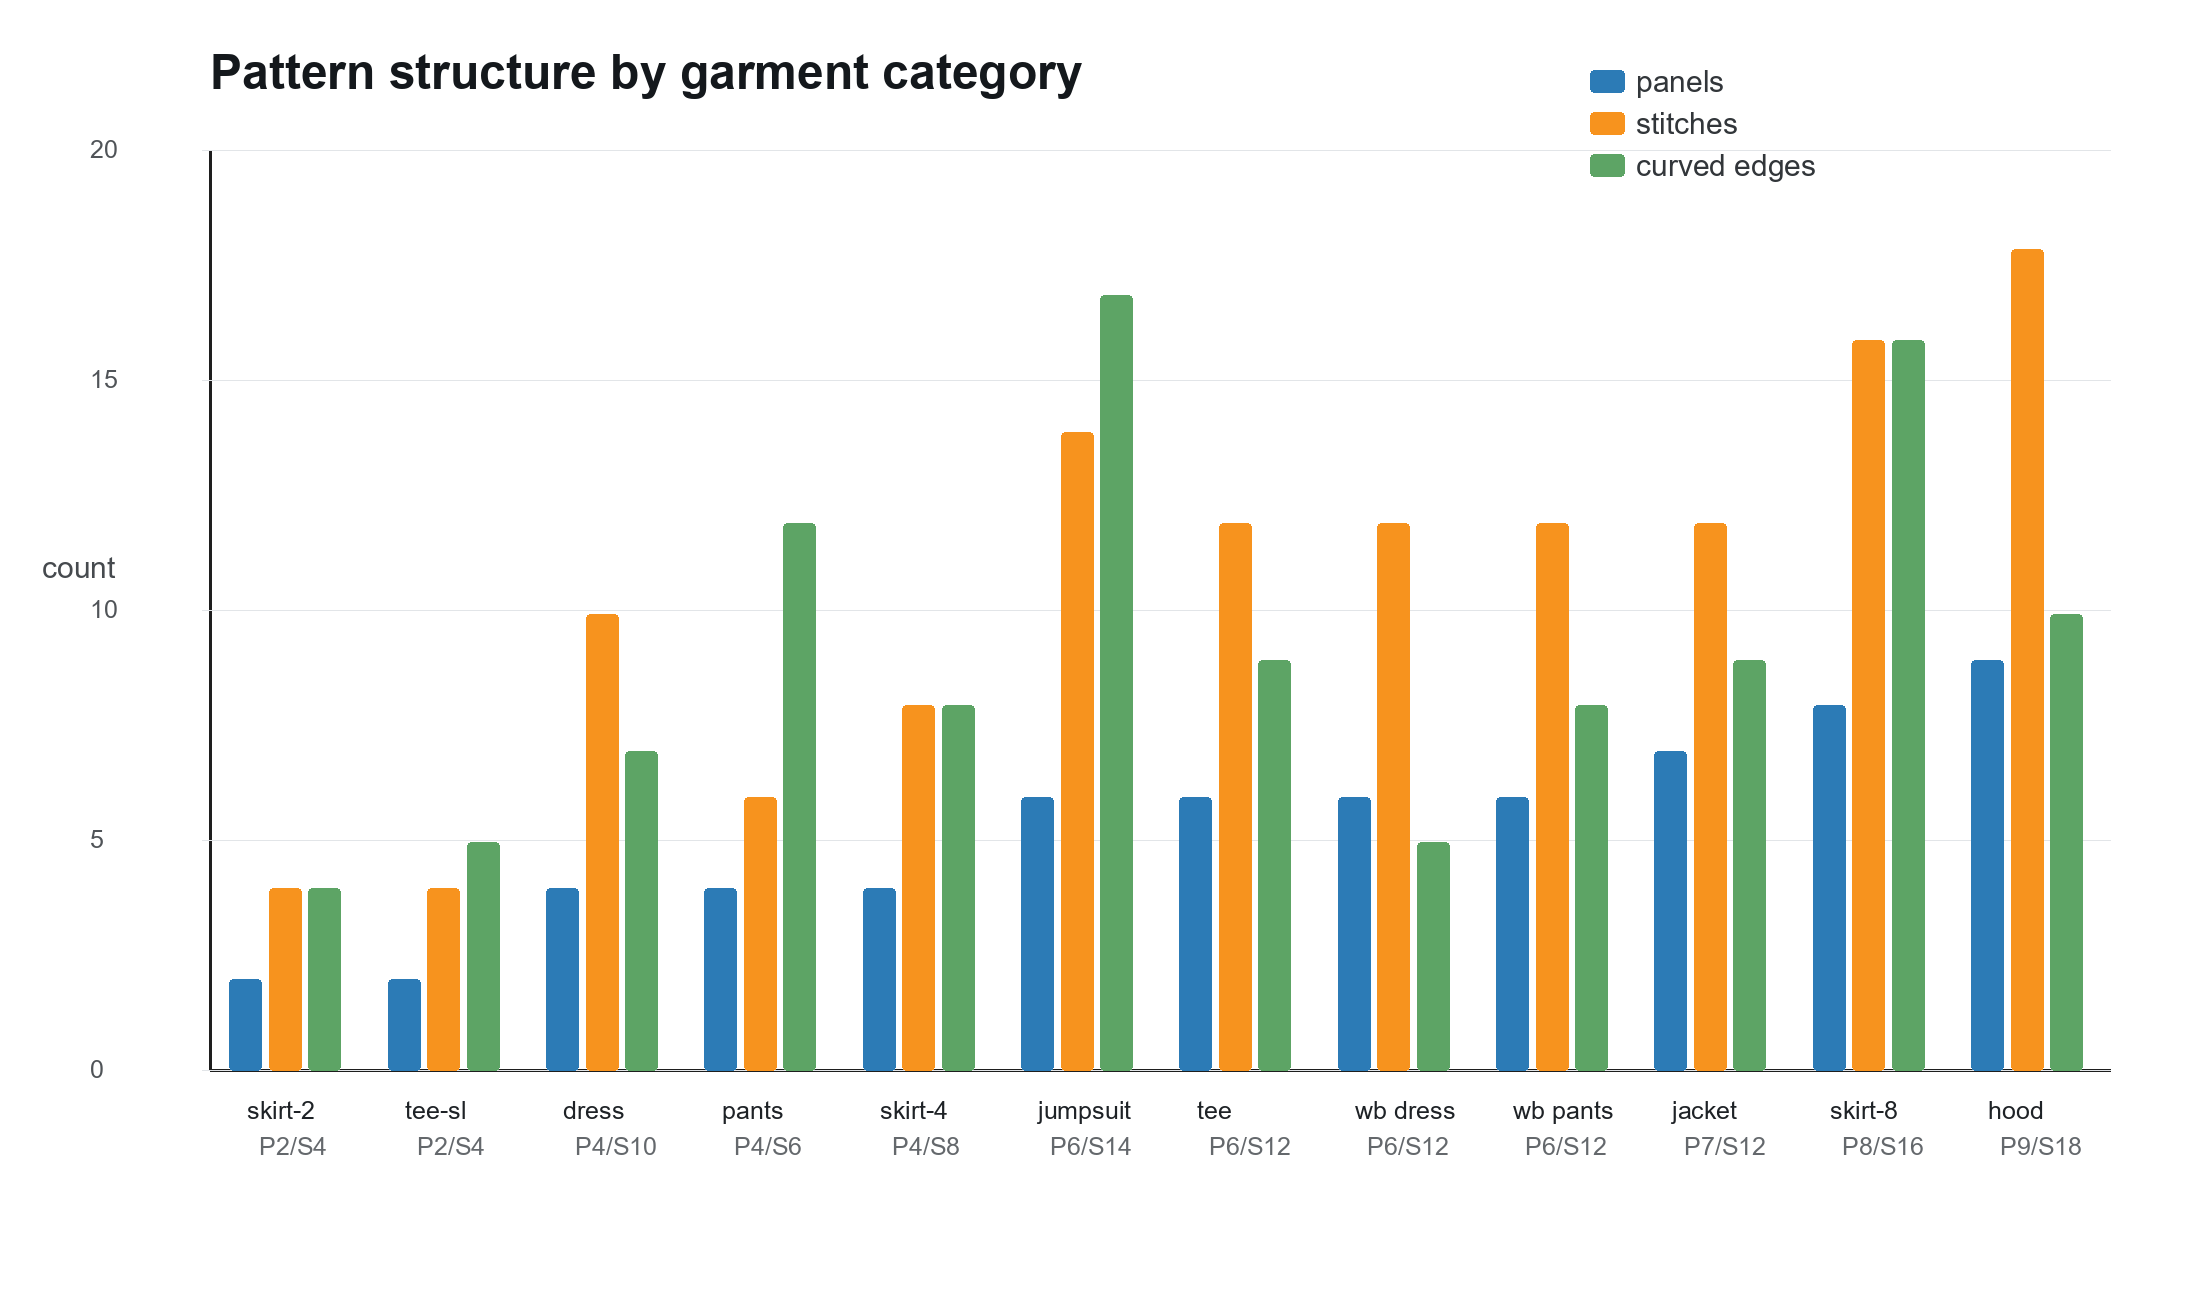
\includegraphics[width=\textwidth]{figures/fig_pattern_structure_by_category.png}
\caption{Pattern-structure summary by garment category. Panels, stitches, and curved edges are parsed from each sample's sewing specification.}
\label{fig:patternstructure}
\end{figure}

\begin{figure}[!htbp]
\centering
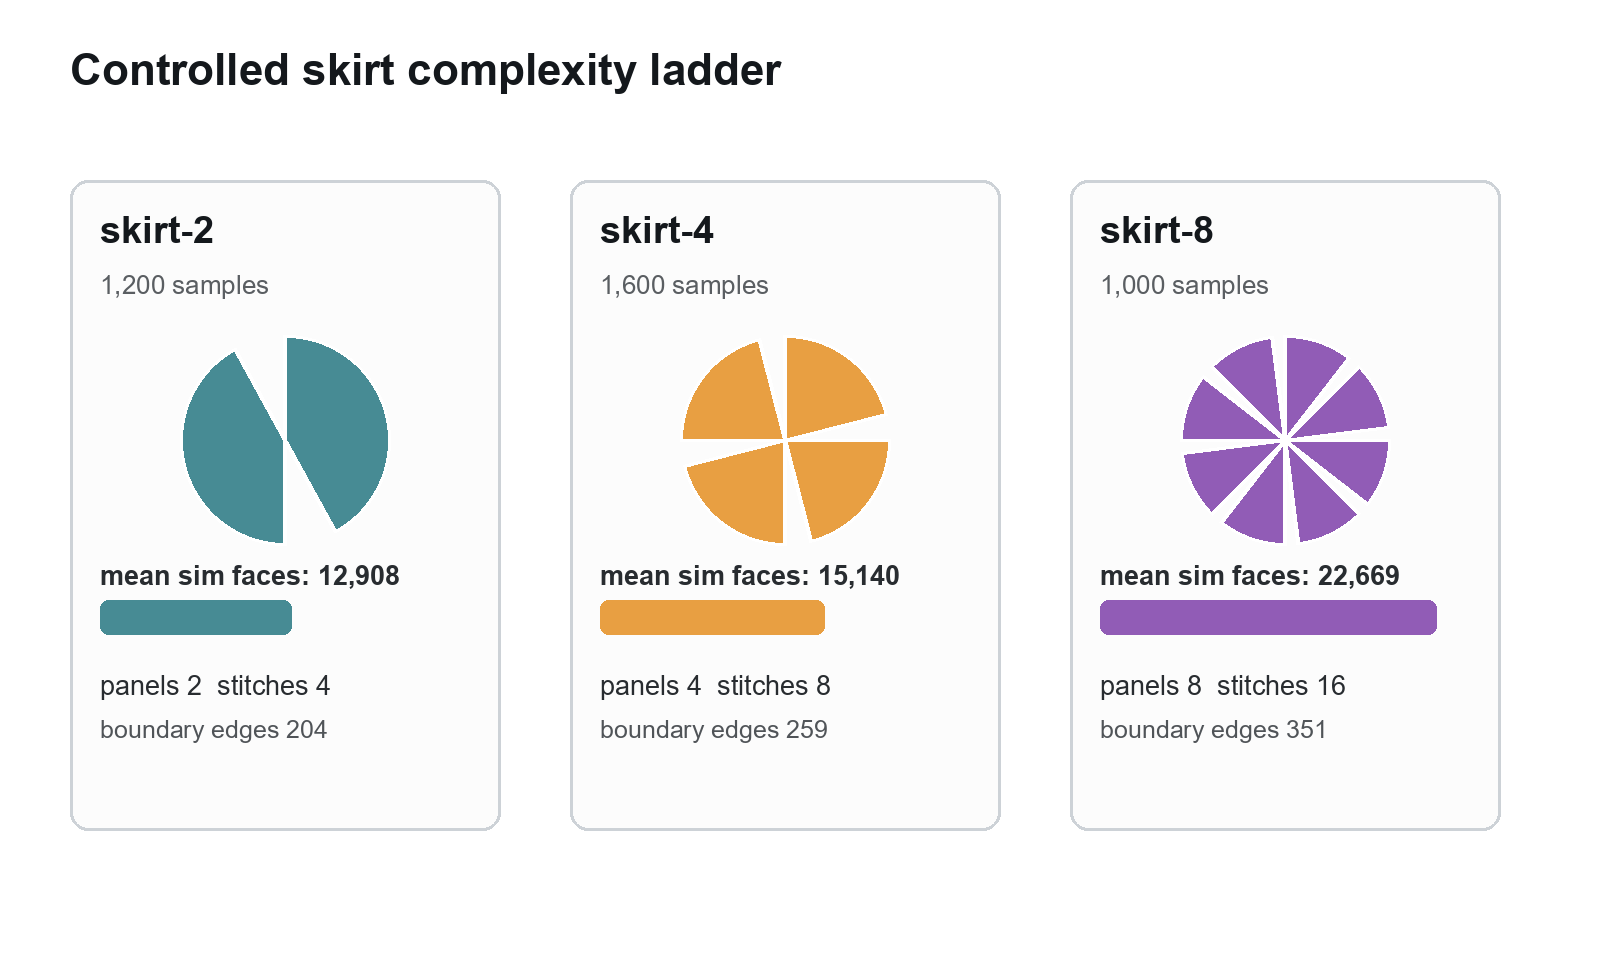
\includegraphics[width=0.95\textwidth]{figures/fig_skirt_complexity_ladder.png}
\caption{Controlled skirt complexity ladder. The skirt families provide a clean within-garment progression from two to four to eight panels, with corresponding increases in stitch count, boundary edges, and mean simulated face count.}
\label{fig:skirtladder}
\end{figure}

\subsubsection{Pattern-Mesh Consistency}

The proposed consistency score is intentionally strict: it requires pattern panels, stitch rules, simulated and scan meshes, zero non-manifold edges, sufficient segmentation labels, and agreement between segmentation length and mesh vertices. Despite this, 22,448 of 22,450 production samples receive a perfect score of 100. The remaining two samples fall below 70 because required mesh and segmentation evidence is absent. The mean production consistency score is 99.996. This result is important for downstream reconstruction work: most samples can be used directly, and the few failures can be isolated deterministically rather than discovered during model training.

\begin{figure}[!htbp]
\centering
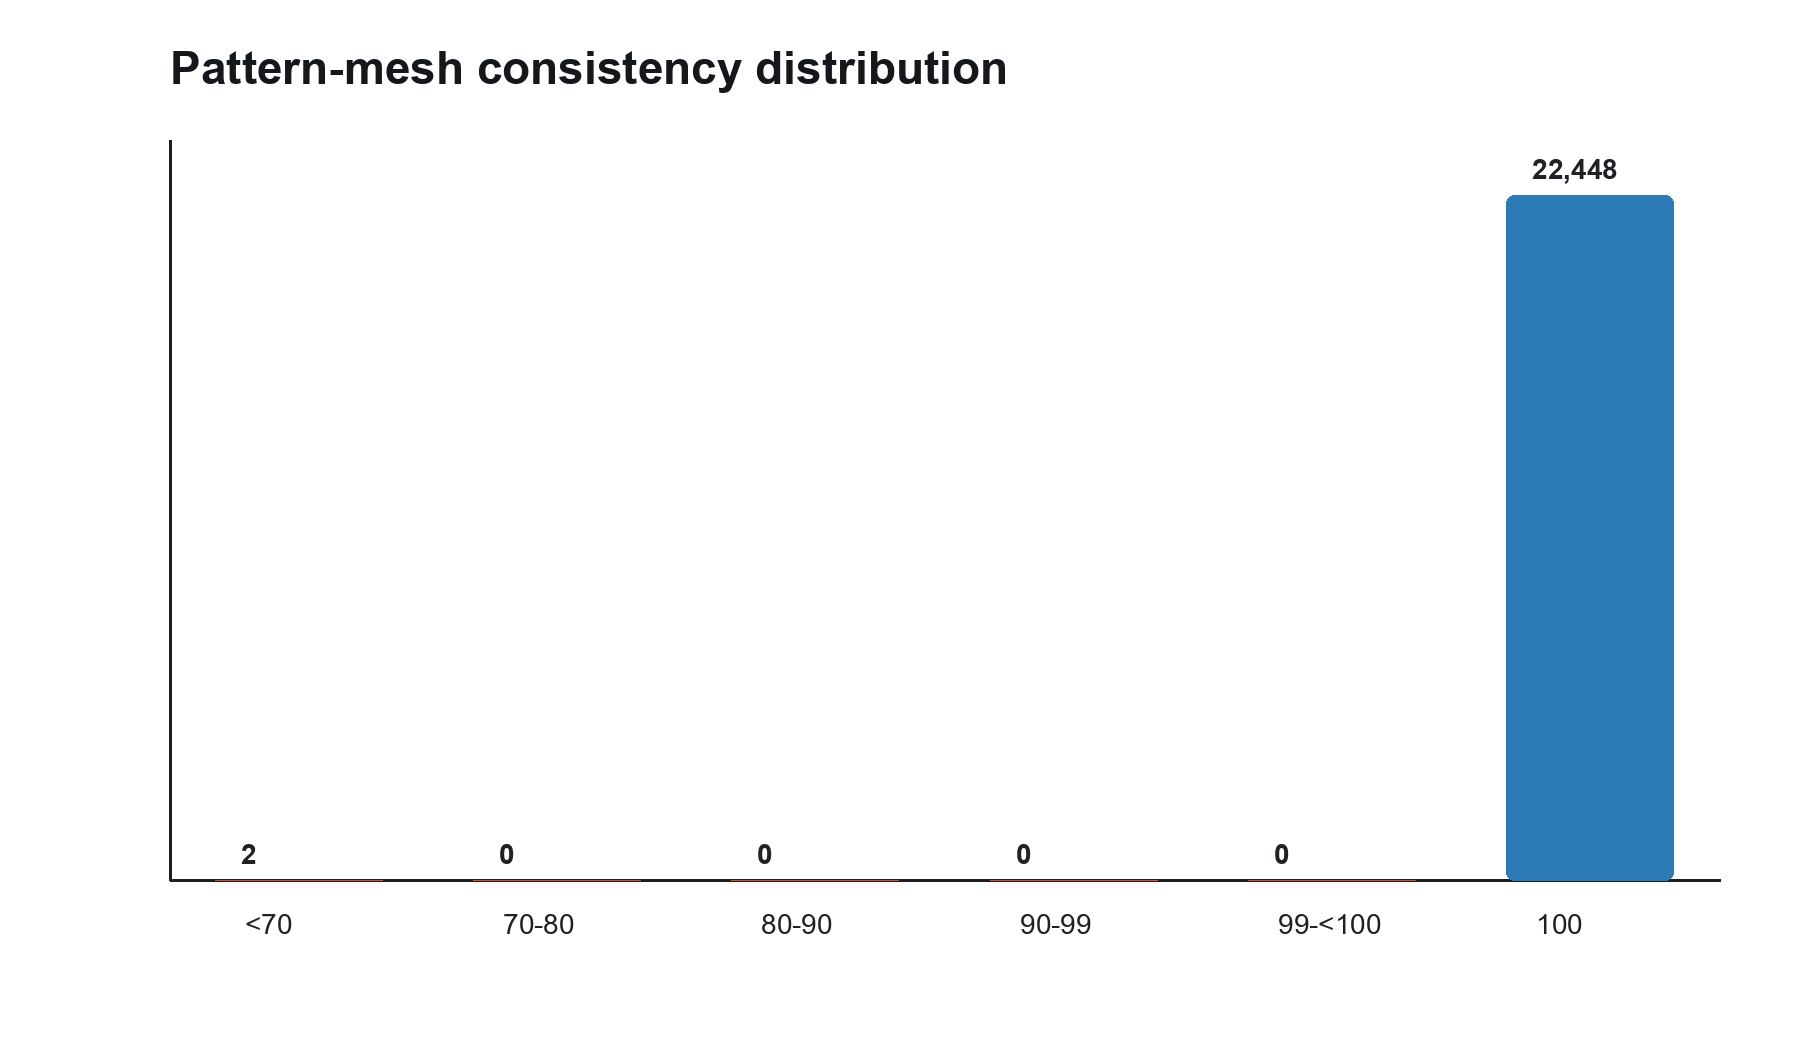
\includegraphics[width=0.95\textwidth]{figures/fig_consistency_histogram.png}
\caption{Pattern-mesh consistency distribution over 22,450 production samples. The score detects two low-consistency samples while 22,448 samples satisfy all implemented consistency checks.}
\label{fig:consistency}
\end{figure}

\begin{figure}[!htbp]
\centering
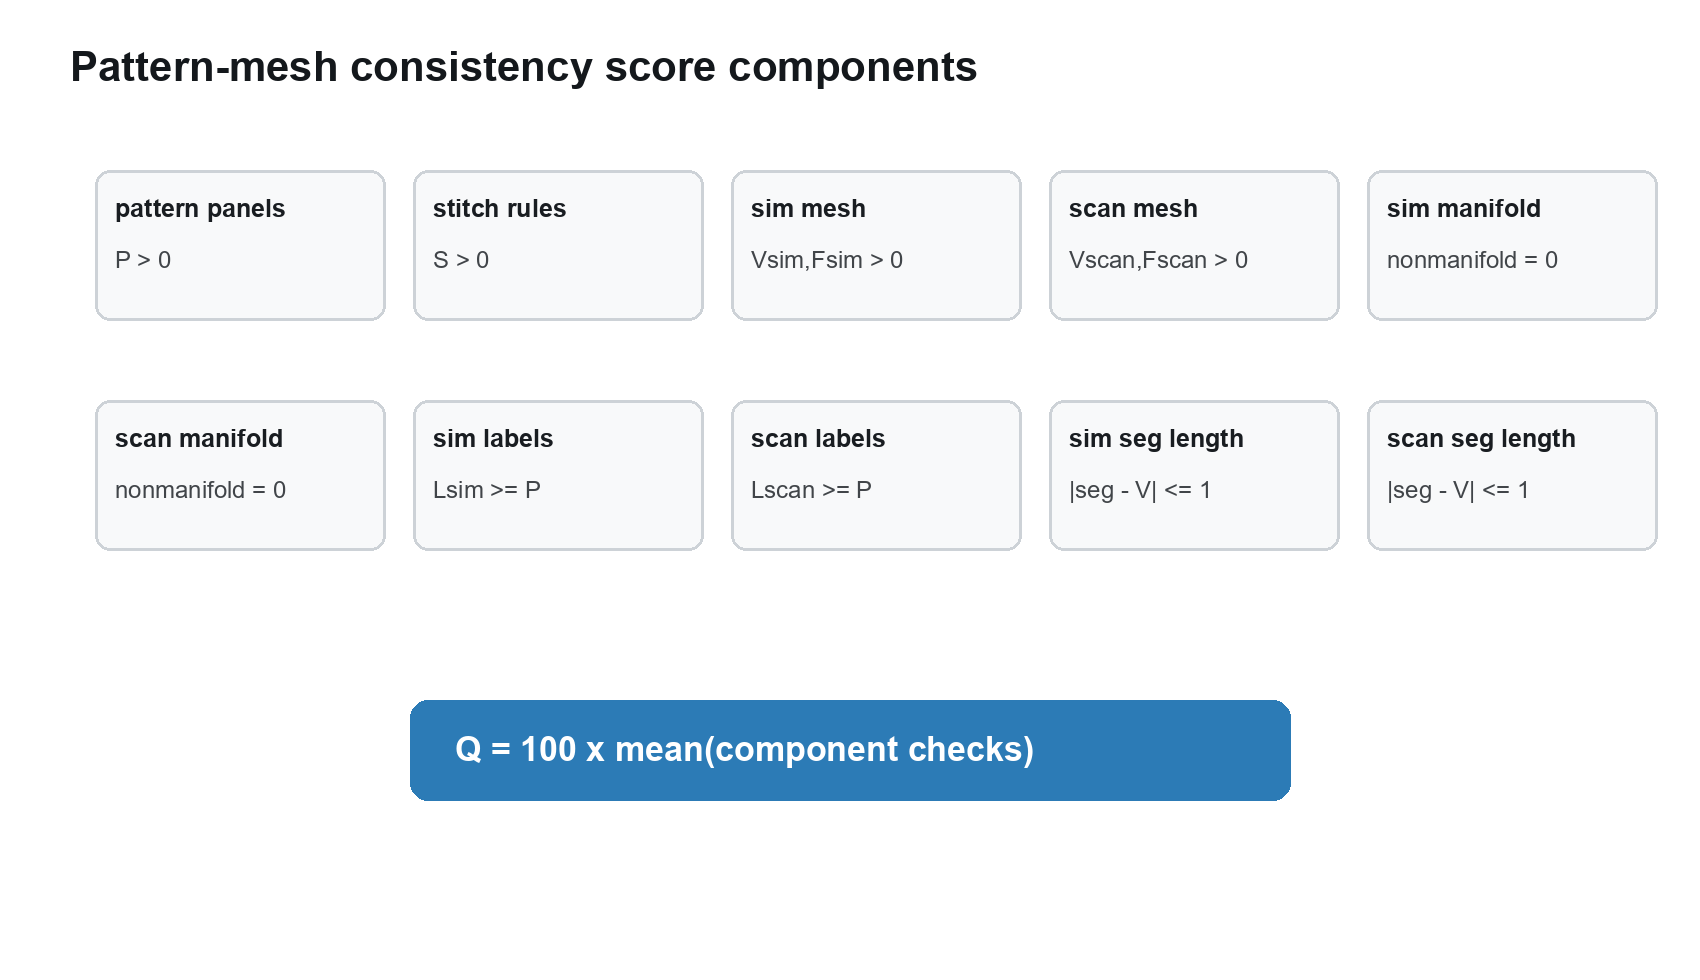
\includegraphics[width=0.95\textwidth]{figures/fig_consistency_components.png}
\caption{Components of the proposed pattern-mesh consistency score. The score acts as a pre-training gate for verifying that pattern, mesh, and segmentation evidence are jointly usable.}
\label{fig:consistencycomponents}
\end{figure}

\subsection{Retrieval and Generalization Results}

\subsubsection{Retrieval and Reconstruction Baselines}

Table~\ref{tab:retrieval} reports retrieval-style reconstruction baselines on the stratified test split. Random category prediction obtains 8.14\% top-1 accuracy and the majority-category baseline obtains 12.02\%. Mesh-only nearest-neighbor retrieval is substantially stronger, reaching 77.32\% top-1, 95.43\% top-5, and 0.850 MRR. Segmentation-only features improve top-1 accuracy to 88.12\%. Pattern-only features reach 100\% because the pattern descriptors expose category-defining template structure. Combined features reach 99.97\% top-1 and near-zero panel and stitch errors.

The reconstruction interpretation is deliberately simple: the nearest training sample supplies the predicted pattern structure for a test query. Under this baseline, mesh-only retrieval has a panel-count MAE of 0.664 and a stitch-count MAE of 1.426. Segmentation-only retrieval nearly eliminates panel error but retains a small stitch-count error. Combined retrieval reduces panel and stitch MAE to below 0.002, with the remaining error caused by one anomalous nearest-neighbor match. These results establish a strong but transparent baseline for later learned image-to-pattern or mesh-to-pattern reconstruction.

\begin{table}[!htbp]
\caption{Retrieval and reconstruction baselines on the stratified test split. MAE is computed between the retrieved training pattern and the ground-truth test pattern.}\label{tab:retrieval}
\centering
\footnotesize
\begin{tabular}{lrrrrrr}
\toprule
Baseline & Features & Test \(N\) & Top-1 & Top-5 & MRR & Panel/Stitch MAE \\
\midrule
Random category & 0 & 3,368 & 0.0814 & 0.4167 & 0.0000 & 0.000/0.000 \\
Majority category & 0 & 3,368 & 0.1202 & 0.5502 & 0.0000 & 0.000/0.000 \\
NN pattern & 9 & 3,368 & 1.0000 & 1.0000 & 1.0000 & 0.000/0.000 \\
NN mesh & 14 & 3,368 & 0.7732 & 0.9543 & 0.8504 & 0.664/1.426 \\
NN segmentation & 8 & 3,368 & 0.8812 & 0.9774 & 0.9235 & 0.005/0.101 \\
NN combined & 31 & 3,368 & 0.9997 & 0.9997 & 0.9997 & 0.001/0.002 \\
\bottomrule
\end{tabular}
\end{table}

\begin{figure}[!htbp]
\centering
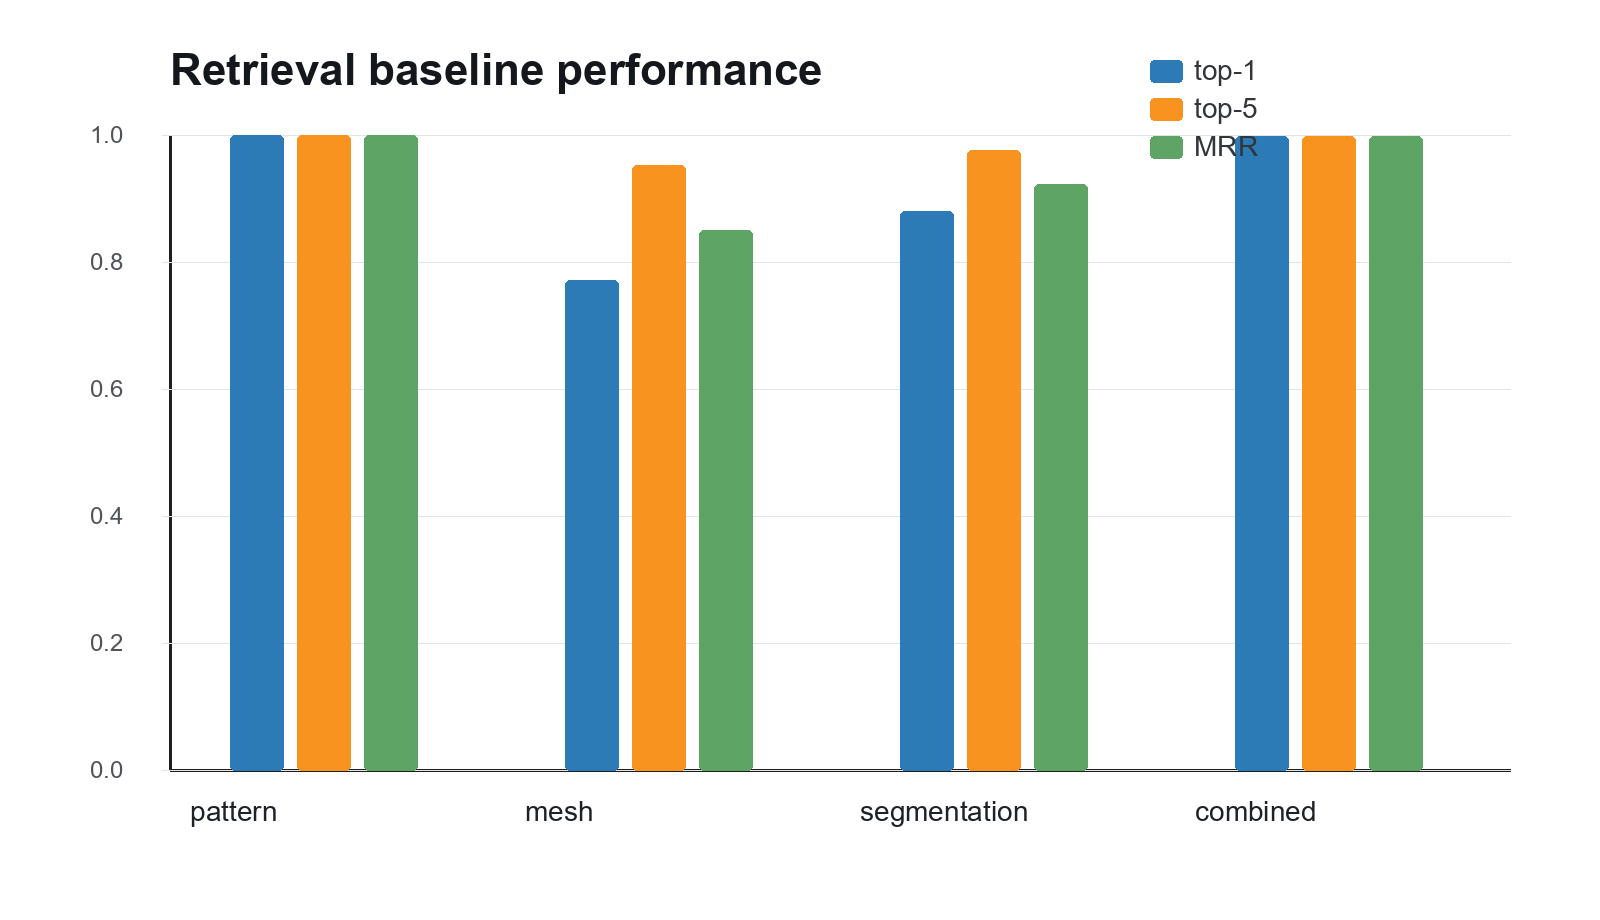
\includegraphics[width=0.95\textwidth]{figures/fig_retrieval_baselines.png}
\caption{Nearest-neighbor retrieval baseline performance. Mesh and segmentation features provide nontrivial category-retrieval baselines, while combined structured features nearly recover the pattern category and panel/stitch structure.}
\label{fig:retrieval}
\end{figure}

\begin{figure}[!htbp]
\centering
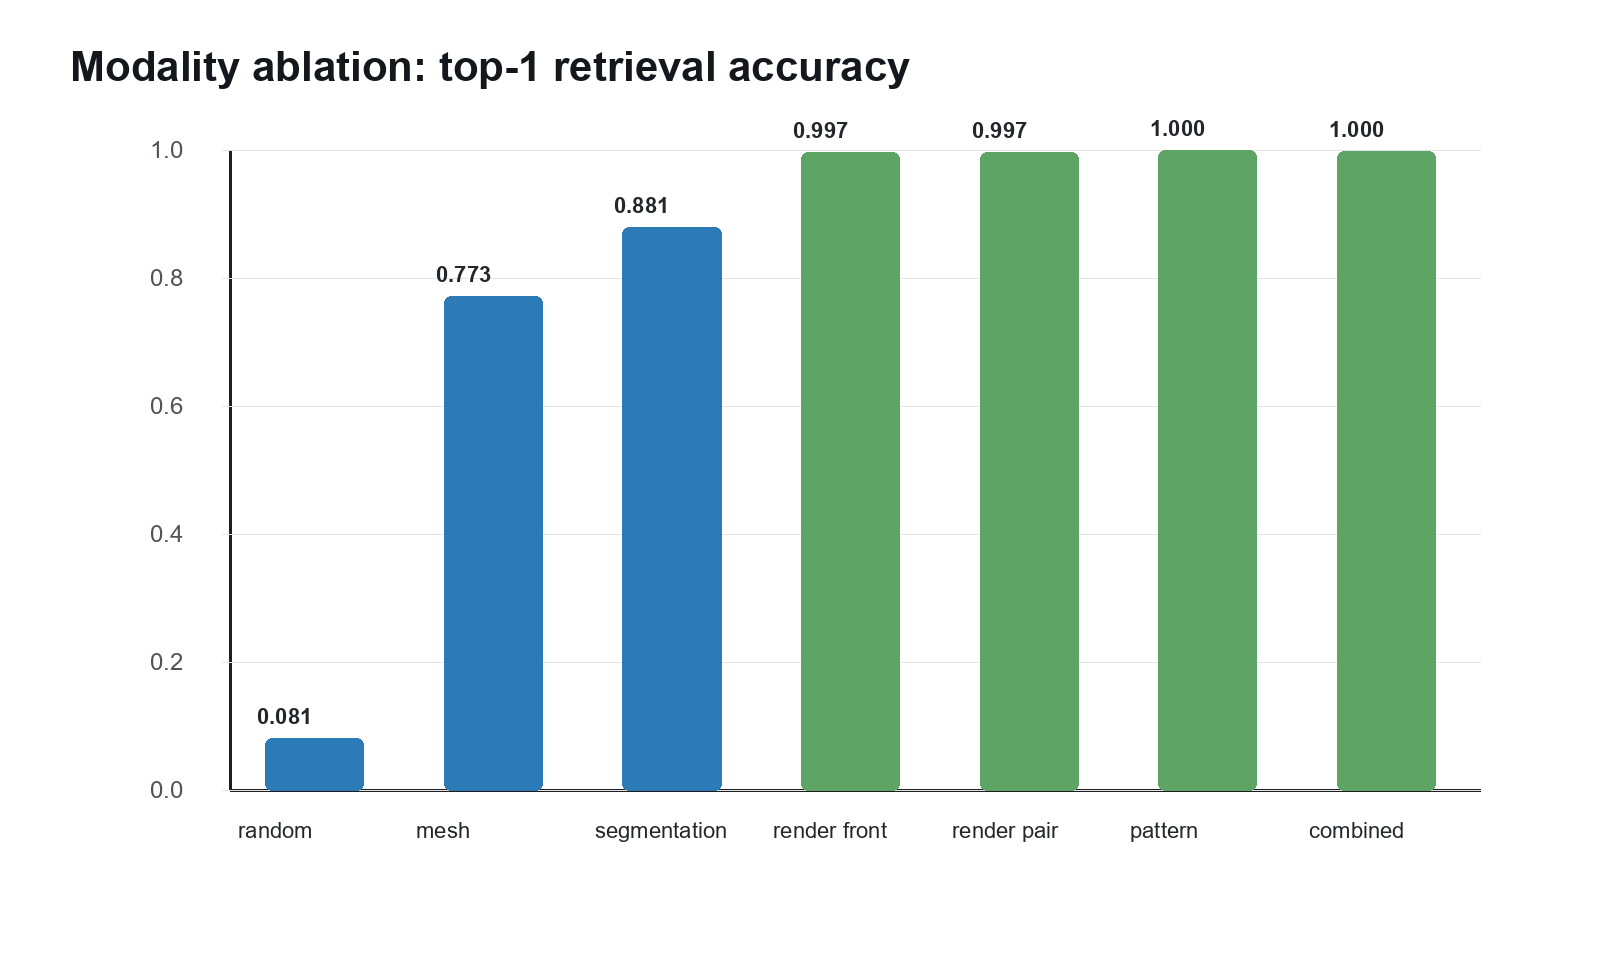
\includegraphics[width=0.95\textwidth]{figures/fig_modality_ablation.png}
\caption{Modality ablation across random, mesh, segmentation, render, pattern, and combined retrieval settings. The comparison separates evidence availability from reconstruction difficulty.}
\label{fig:modalityablation}
\end{figure}

\subsubsection{Render-to-Pattern Retrieval Baseline}

Table~\ref{tab:renderretrieval} reports deterministic render-image retrieval on the same split. Front-view descriptors alone achieve 99.73\% top-1 accuracy and 99.97\% top-5 accuracy. Back-view descriptors perform similarly. The paired front-back descriptor reaches 99.70\% top-1 accuracy and 99.97\% top-5 accuracy. Panel and stitch errors are near zero because nearest rendered neighbors almost always come from the correct category and template family.

This result has two interpretations. First, the dataset is highly suitable for controlled render-to-pattern retrieval experiments because rendered appearance, category, and pattern structure are strongly coupled. Second, the result reveals an important benchmark caveat: high retrieval accuracy from deterministic image descriptors can reflect template and rendering regularity, not necessarily deep understanding of garment construction. Future image-to-pattern models should therefore compare against this simple render baseline and should report cross-template or cross-style splits when claiming generalization beyond the dataset's template families.

\begin{table}[!htbp]
\caption{Render-image nearest-neighbor retrieval baselines on the same stratified test split.}\label{tab:renderretrieval}
\centering
\footnotesize
\begin{tabular}{lrrrrrr}
\toprule
Baseline & Features & Test \(N\) & Top-1 & Top-5 & MRR & Panel/Stitch MAE \\
\midrule
NN front render & 375 & 3,368 & 0.9973 & 0.9997 & 0.9985 & 0.006/0.009 \\
NN back render & 375 & 3,368 & 0.9973 & 0.9994 & 0.9983 & 0.006/0.010 \\
NN front+back render & 1,125 & 3,368 & 0.9970 & 0.9997 & 0.9983 & 0.005/0.011 \\
\bottomrule
\end{tabular}
\end{table}

\begin{figure}[!htbp]
\centering
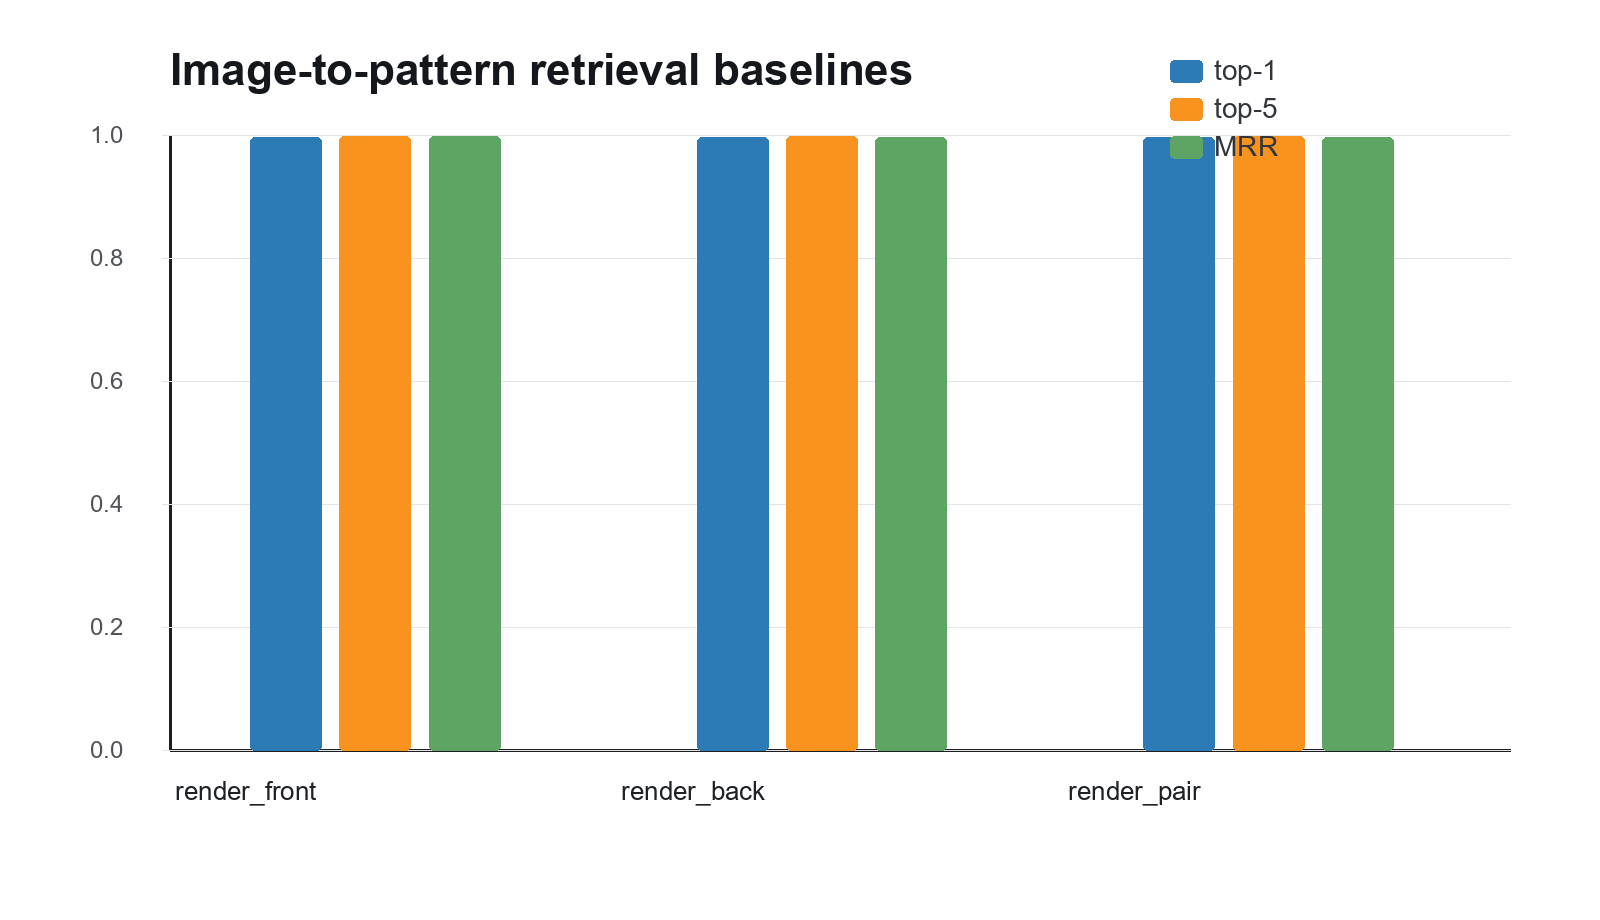
\includegraphics[width=0.95\textwidth]{figures/fig_image_retrieval_baselines.png}
\caption{Render-image retrieval baseline performance. Simple deterministic image descriptors are already strong on the category-level retrieval task, indicating that rendered appearance and pattern-template identity are tightly coupled in this corpus.}
\label{fig:renderbaseline}
\end{figure}

\begin{figure}[!htbp]
\centering
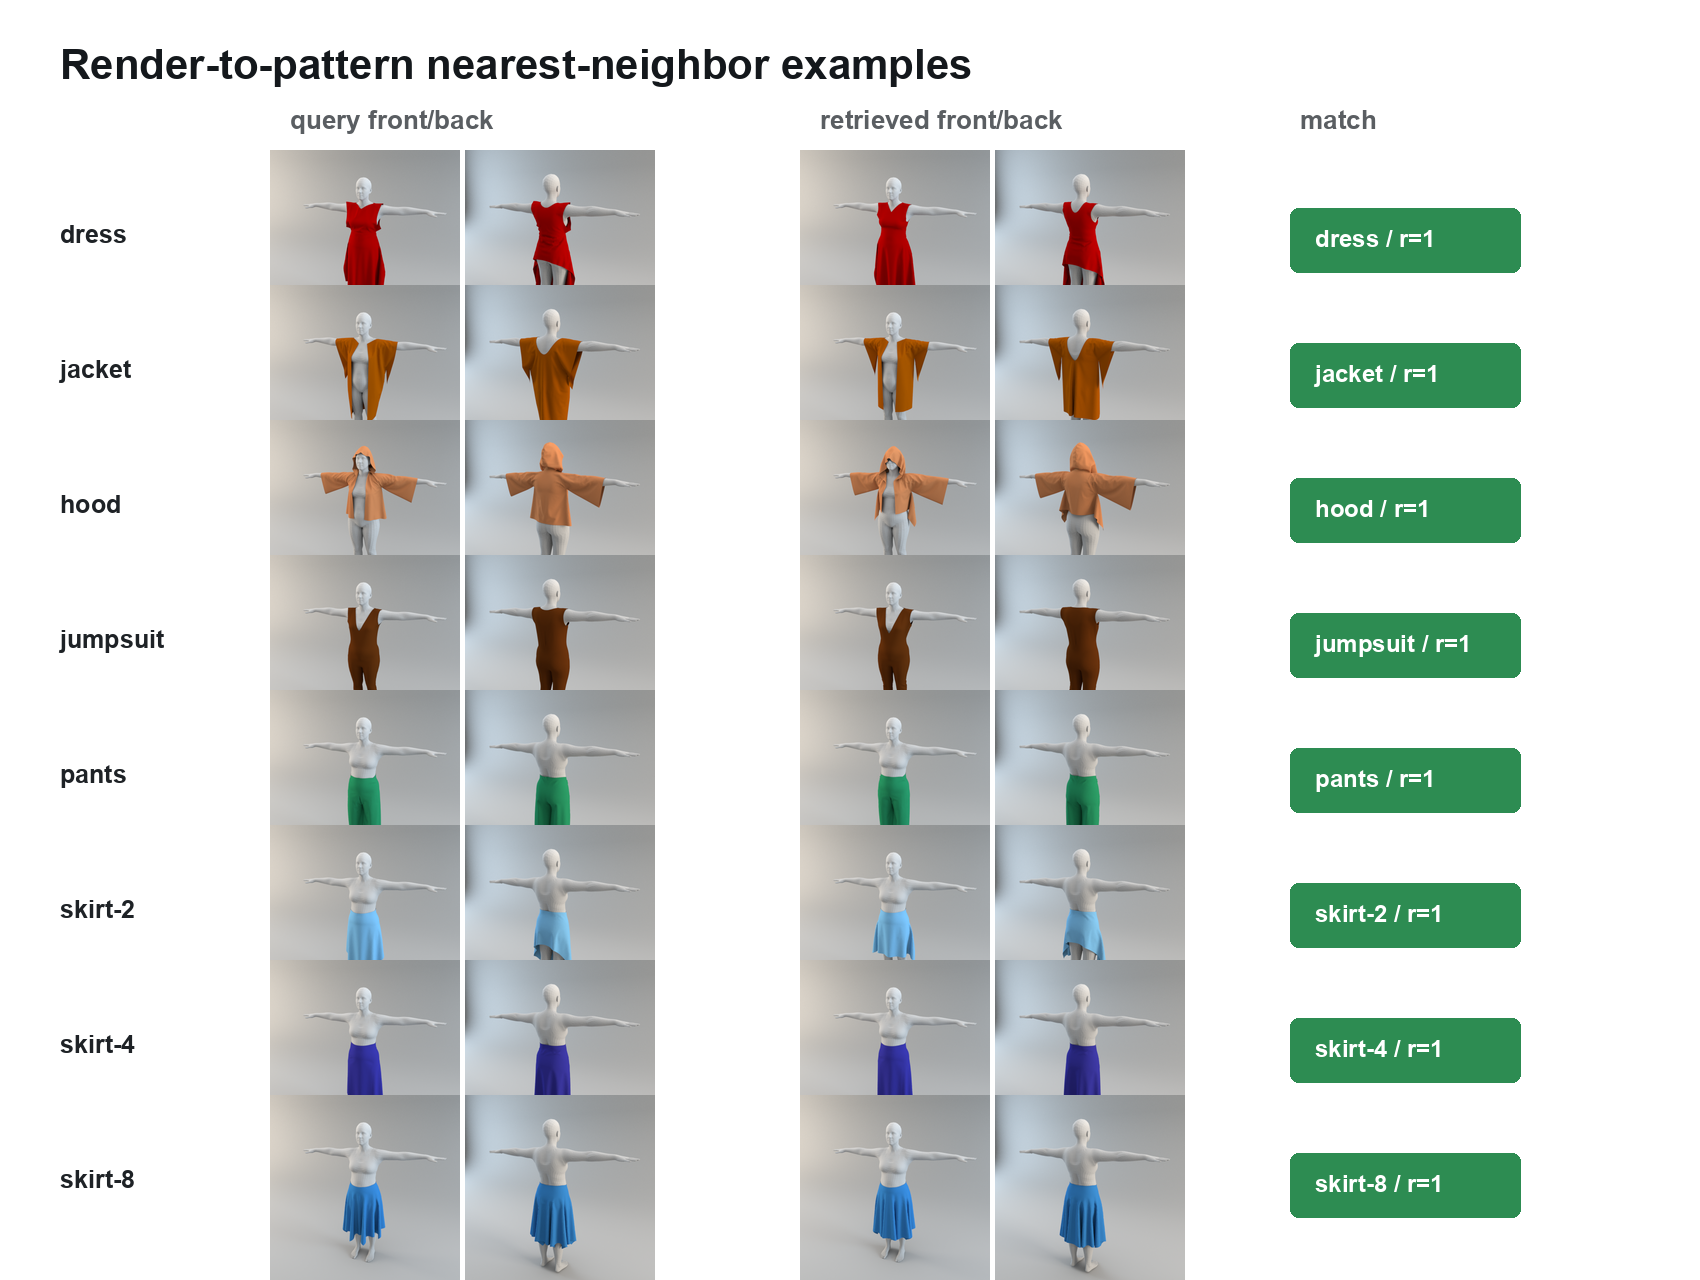
\includegraphics[width=\textwidth,height=0.86\textheight,keepaspectratio]{figures/fig_image_retrieval_examples.png}
\caption{Qualitative render-to-pattern nearest-neighbor examples. Each row shows a test query's front/back render pair and the retrieved training neighbor's front/back render pair. The rank reports the first retrieved neighbor from the true category.}
\label{fig:renderexamples}
\end{figure}

\subsubsection{Render Retrieval Error Analysis}

The paired render baseline makes only ten top-1 category errors on 3,368 test samples. Figure~\ref{fig:rendererrors} shows these errors. They are not arbitrary: two jacket samples retrieve tees, two tee samples retrieve jackets, one tee retrieves a sleeveless tee, pants and waistband pants are confused in both directions, one eight-panel skirt retrieves straight pants, and one waistband dress retrieves a jumpsuit. In each case, the correct category is still close in the ranking, typically rank two or three. The only larger failure is the eight-panel skirt case, where the true category appears at rank six because the visible lower-body silhouette is weak in the resized descriptor.

This pattern supports a useful failure taxonomy. First, upper-body silhouettes can dominate sleeve and torso distinctions, causing jacket--tee confusion. Second, waistband variants can be visually subtle in low-resolution image descriptors even though they are structurally different in the sewing pattern. Third, full-body garments such as jumpsuits and waistband dresses can be visually close when the descriptor emphasizes global color and silhouette. These failures motivate reporting both retrieval metrics and qualitative nearest-neighbor evidence in future image-to-pattern papers.

\begin{figure}[!htbp]
\centering
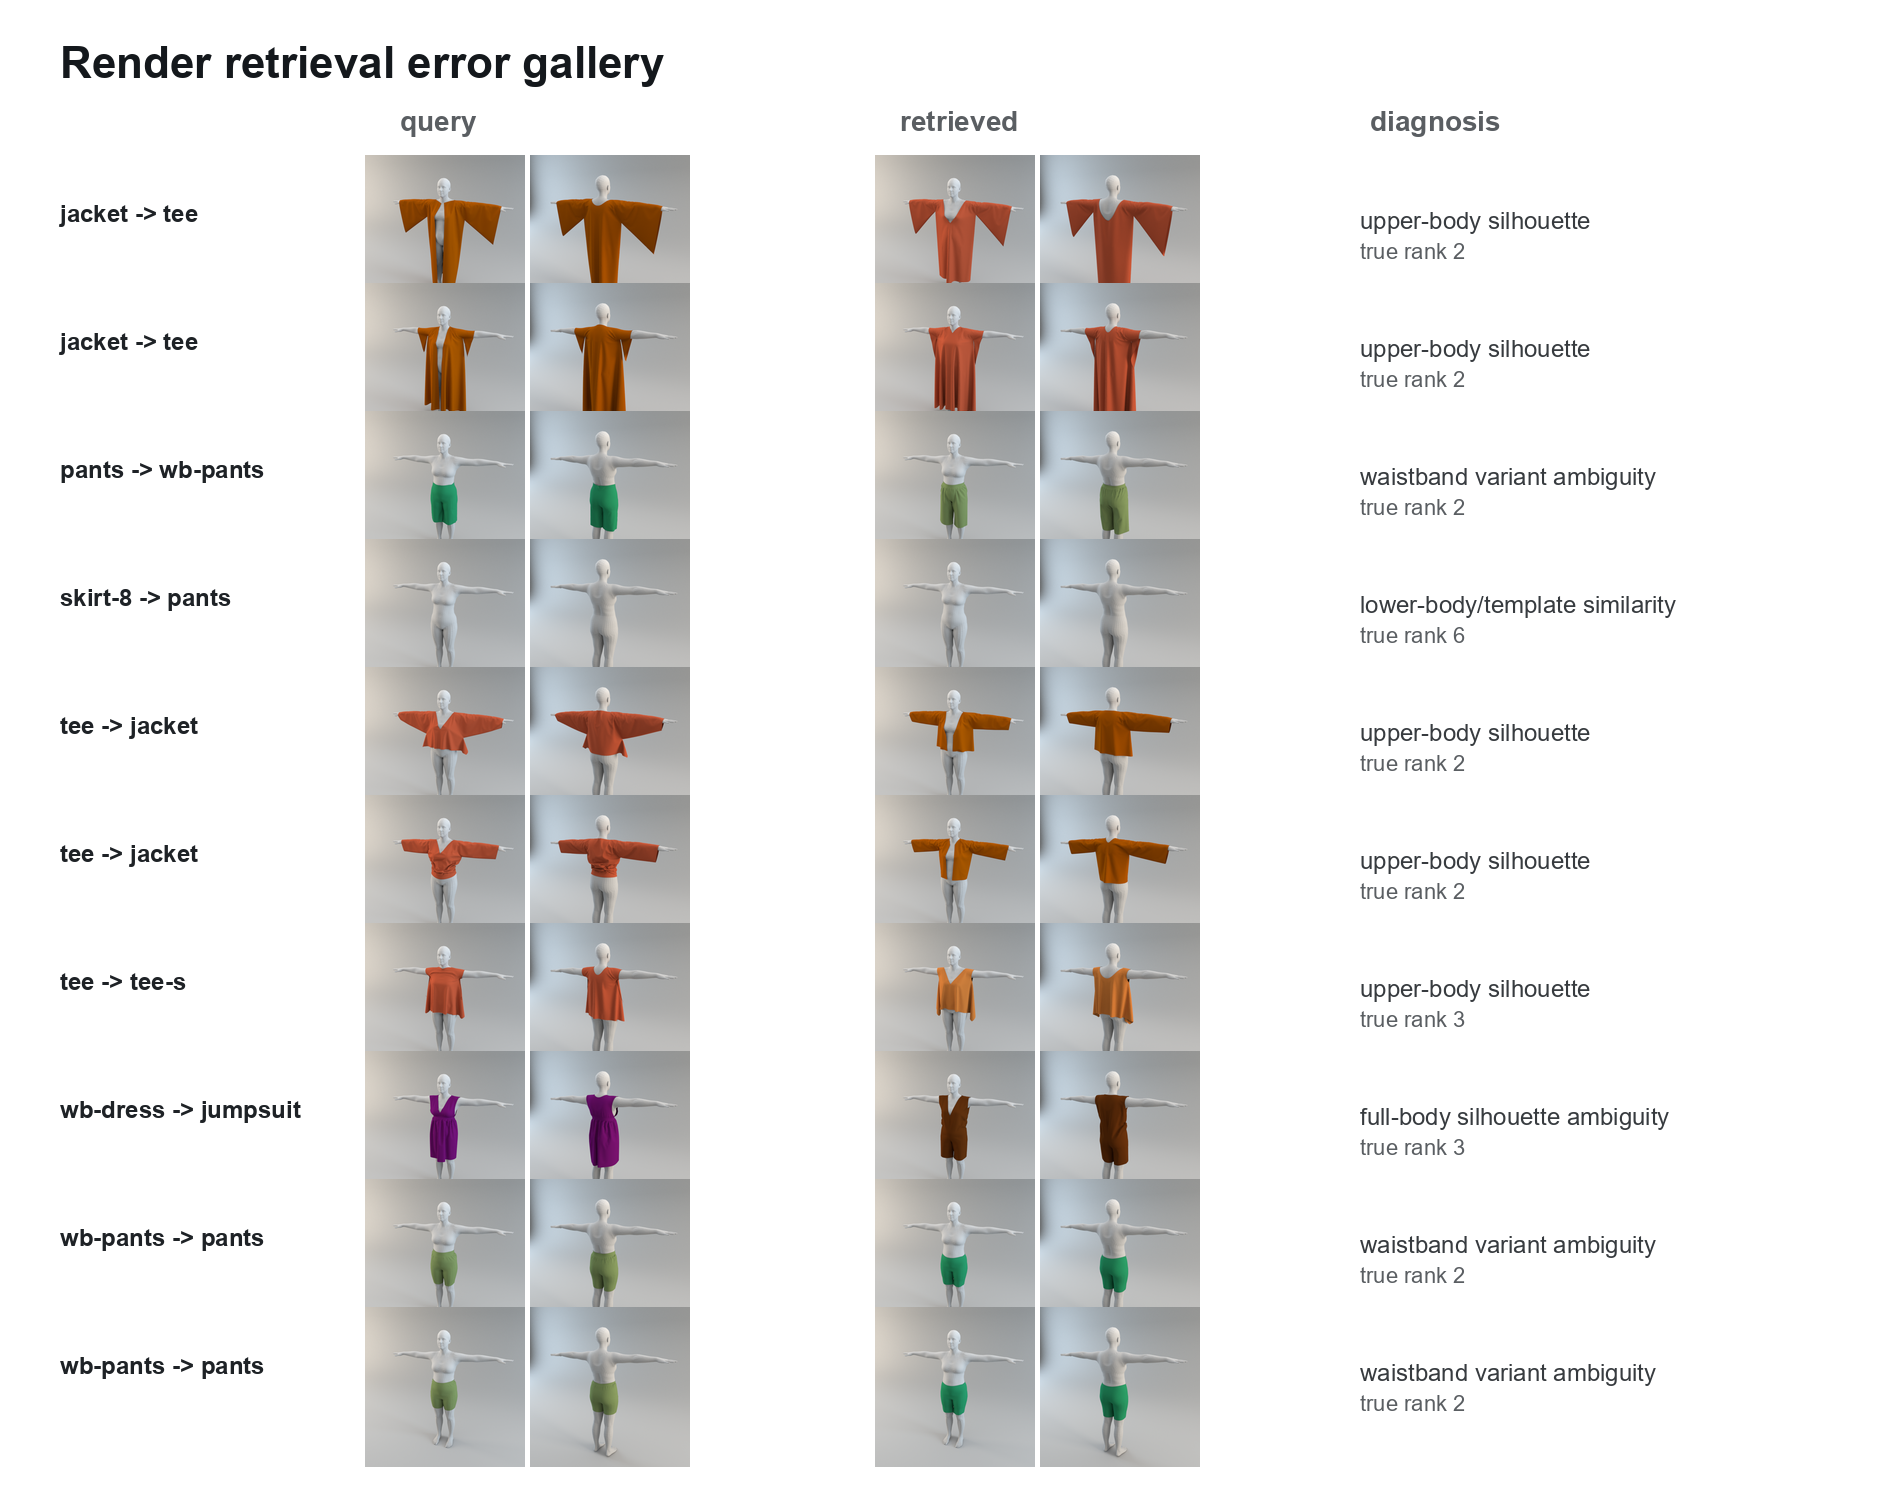
\includegraphics[width=\textwidth,height=0.86\textheight,keepaspectratio]{figures/fig_render_error_gallery.png}
\caption{All top-1 errors made by the paired render-image retrieval baseline. The errors concentrate in visually similar garment families, and the true category remains close in the nearest-neighbor ranking.}
\label{fig:rendererrors}
\end{figure}

\subsubsection{Hard-Generalization Analysis}

The high in-distribution retrieval scores should not be read as evidence that sewing-pattern reconstruction is solved. Table~\ref{tab:hardgeneralization} reports harder tests that remove exact category matches or perturb the render descriptor. In leave-one-category-out evaluation, structured descriptors preserve panel counts better than render descriptors, reaching 60.64\% mean panel-exact transfer and 49.87\% mean stitch-exact transfer. Render descriptors retain stronger family-level transfer, at 52.92\%, but fall to 13.14\% panel-exact and 15.29\% stitch-exact transfer. This contrast is expected: render appearance is useful for visual family matching, whereas pattern/mesh/segmentation descriptors encode more direct construction evidence.

Paired transfer is stricter because the training index contains only one related source category. It exposes deterministic structural gaps between variants. For example, straight-side pants to waistband pants has a two-panel and six-stitch difference, jacket to hooded jacket has a two-panel and six-stitch difference, and tee to sleeveless tee has a four-panel and eight-stitch difference. The nearest-neighbor family match is perfect in these paired settings, but panel-exact and stitch-exact transfer are zero because the held-out target category changes the sewing template itself.

The render-noise stress test further clarifies the role of controlled rendering. With no perturbation, the paired render descriptor obtains 99.70\% top-1 accuracy on the stratified split. Adding Gaussian descriptor noise with \(\sigma=0.05\) reduces top-1 accuracy to 12.53\%, and larger perturbations remain near the 12--13\% range. These results support a conservative benchmark interpretation: the original render split is valuable as an in-distribution retrieval baseline, while claims about general image-to-pattern reconstruction should use additional domain-shift, held-template, or real-photo protocols.

\begin{table}[!htbp]
\caption{Hard-generalization summary. Leave-one-category-out results are averaged over 12 held-out categories. Render-noise rows use the original stratified split with perturbed test descriptors.}\label{tab:hardgeneralization}
\centering
\footnotesize
\begin{tabular}{llrrrr}
\toprule
Protocol & Feature set & Family & Panel exact & Stitch exact & Panel/Stitch MAE \\
\midrule
Leave-one-category-out & Structured & 0.2342 & 0.6064 & 0.4987 & 0.644/1.452 \\
Leave-one-category-out & Render pair & 0.5292 & 0.1314 & 0.1529 & 2.918/5.892 \\
Render noise, \(\sigma=0.00\) & Render pair & 0.9985 & 0.9973 & 0.9982 & 0.005/0.011 \\
Render noise, \(\sigma=0.05\) & Render pair & 0.2337 & 0.2007 & 0.1793 & 2.672/5.065 \\
Render noise, \(\sigma=0.35\) & Render pair & 0.2283 & 0.2034 & 0.1948 & 2.649/4.992 \\
\bottomrule
\end{tabular}
\end{table}

\begin{figure}[!htbp]
\centering
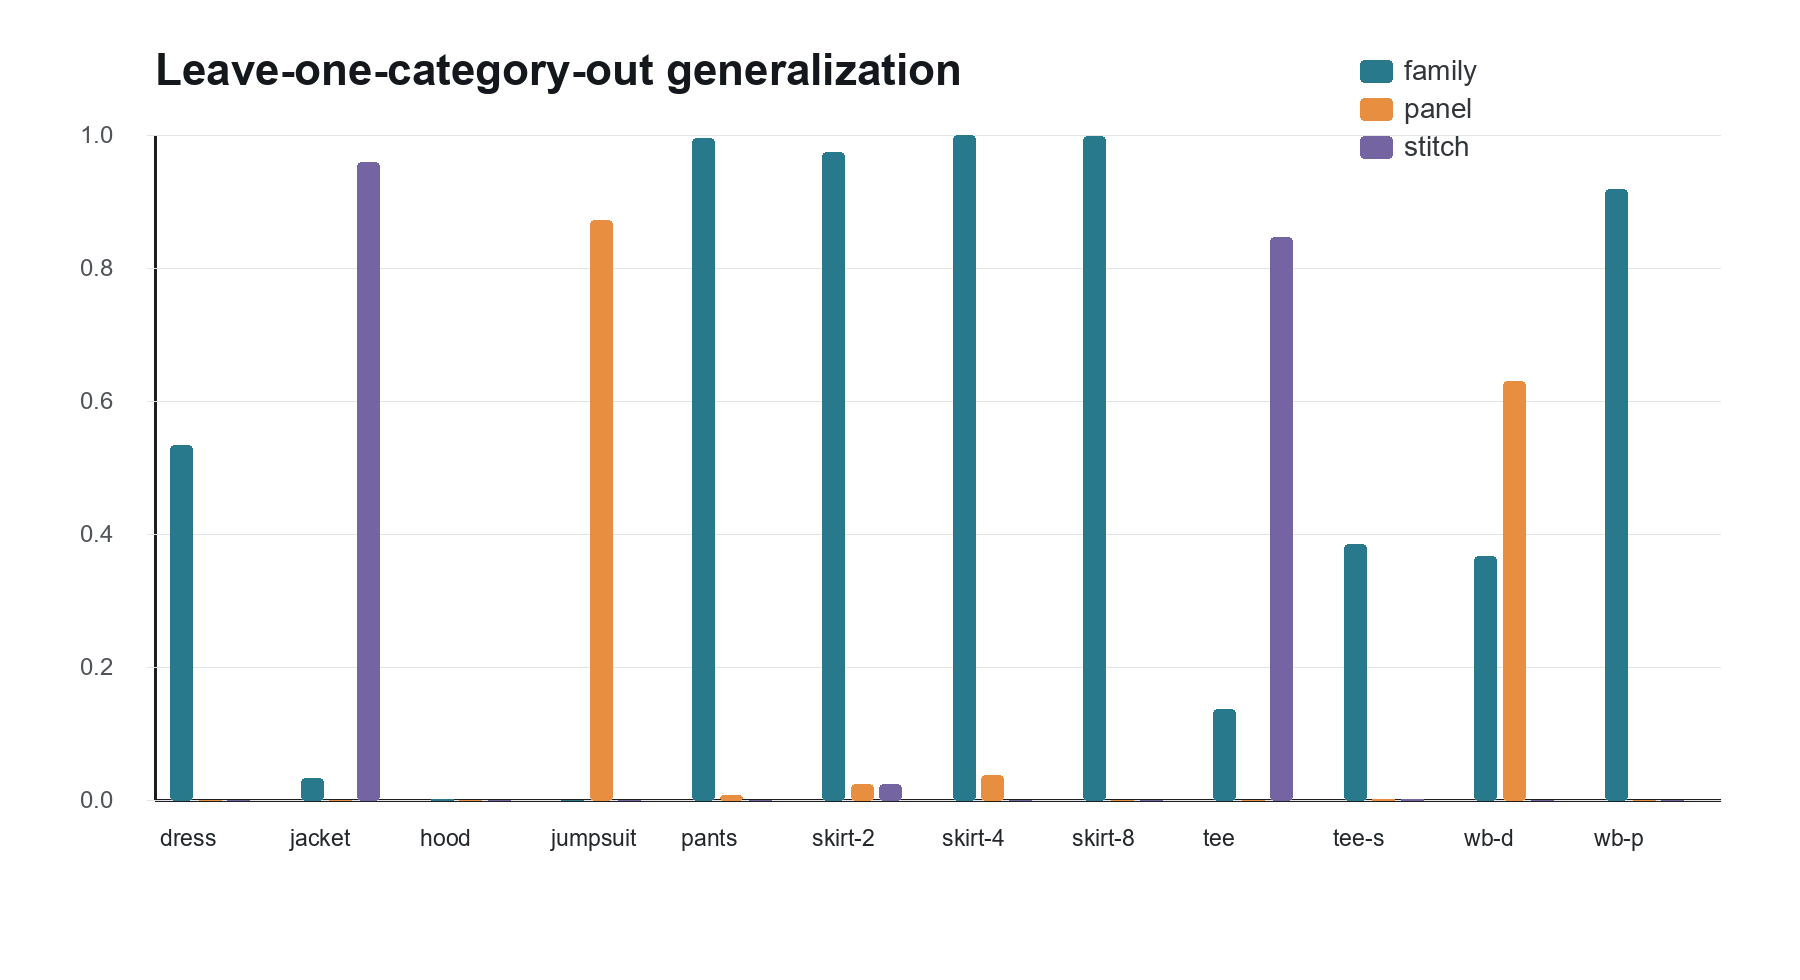
\includegraphics[width=0.95\textwidth]{figures/fig_leave_one_category_out.png}
\caption{Leave-one-category-out transfer for render-pair descriptors. Exact category retrieval is impossible in this protocol because the held-out category is absent from the training index; the plot therefore reports family-level, panel-exact, and stitch-exact transfer.}
\label{fig:loco}
\end{figure}

\begin{figure}[!htbp]
\centering
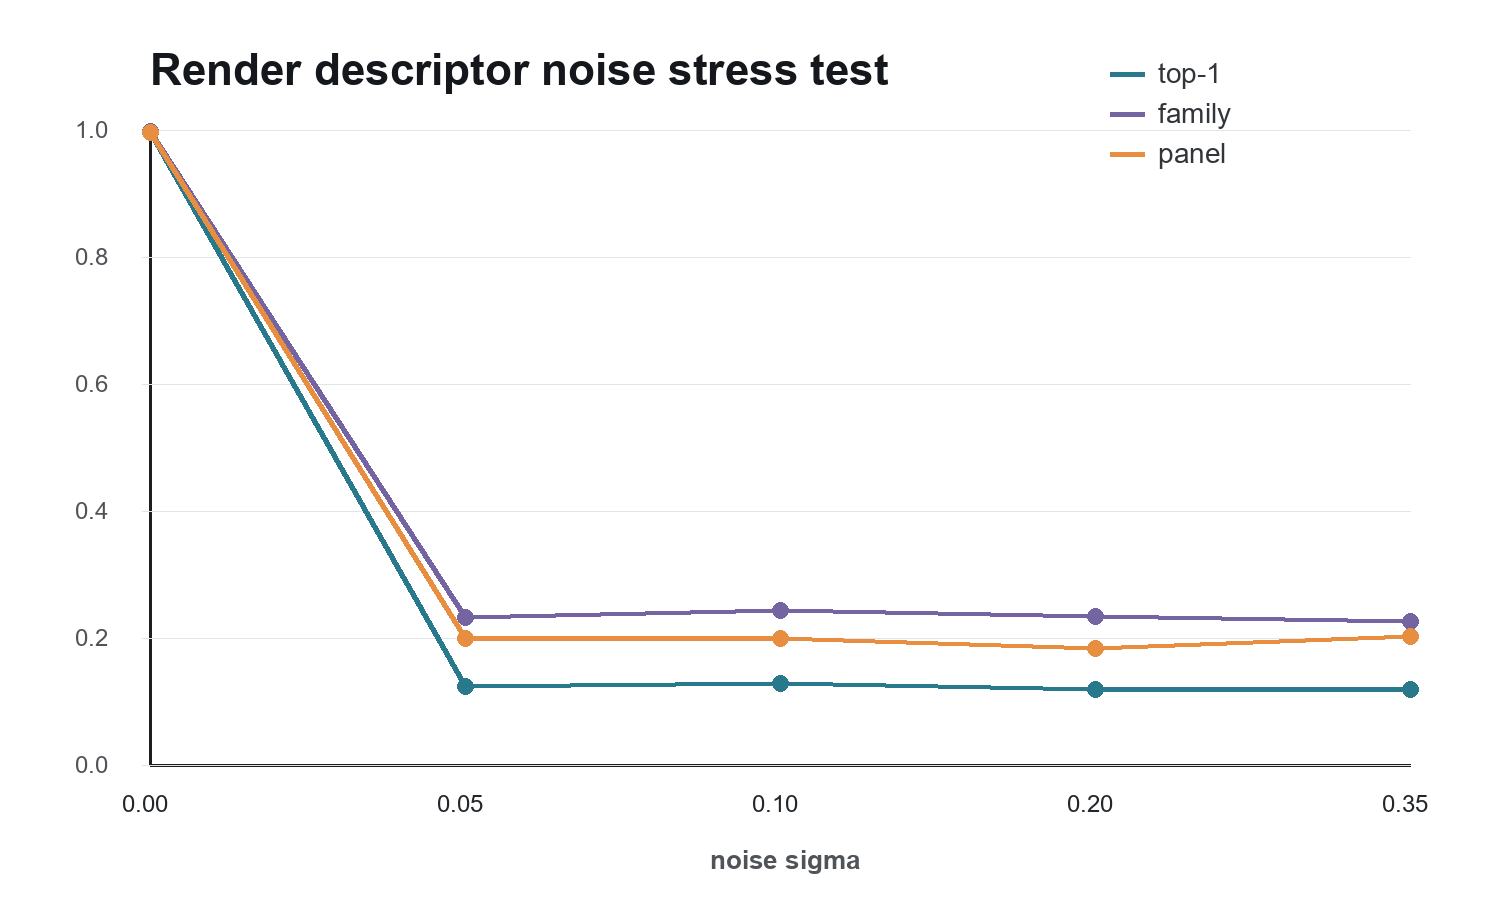
\includegraphics[width=0.95\textwidth]{figures/fig_render_noise_stress.png}
\caption{Render-descriptor noise stress test on the original stratified split. The sharp drop from the clean descriptor to the perturbed descriptor shows that the high render-retrieval score depends on stable controlled-view appearance.}
\label{fig:noisestress}
\end{figure}

\section{Discussion}\label{sec:discussion}

The full experiment supports the use of this corpus as a foundation for sewing-pattern reconstruction research. Unlike image-only clothing datasets such as DeepFashion3D, which are valuable for garment reconstruction but do not expose full sewing-pattern structure \cite{deepfashion3d}, the audited corpus pairs rendered views with editable pattern and stitch evidence. This makes it directly relevant to methods that infer or generate patterns, such as NeuralTailor, Neural Sewing Machines, Panelformer, SewFormer, Design2GarmentCode, and GarmentDiffusion \cite{neuraltailor2022,nsm2022,panelformer2024,sewformer2023,design2garmentcode2025,garmentdiffusion2025}. The comparison also clarifies why the present paper emphasizes data evidence and benchmark controls rather than a new neural architecture.

The category spread also matters. A subset containing only pants and skirts can support basic mesh-pattern studies, but it cannot test the pattern complexity needed for sleeves, jackets, hoods, waistband garments, or multi-panel combinations. The full audit shows a natural difficulty ladder: two-panel skirts and sleeveless tees are structurally simple, while hooded jackets combine high panel count, high stitch count, and high mesh complexity. The full mesh-quality pass adds geometric evidence to this claim: categories differ not only in panel/stitch counts but also in simulated and scan-imitation face counts, boundary-edge structure, and segmentation coverage. This ladder can be used to design curriculum-style experiments for image-to-pattern retrieval or pattern-structure prediction.

The retrieval baselines clarify the difference between dataset usability and reconstruction difficulty. Pattern descriptors almost perfectly identify category because they encode the target structure. Mesh-only retrieval, however, is not trivial: top-1 accuracy remains at 77.32\%, indicating that geometric features alone confuse categories with related body coverage or mesh resolution. Segmentation features are more informative than mesh statistics, reaching 88.12\% top-1, because panel labels encode a closer proxy to sewing structure. These results suggest that future learned reconstruction methods should report separate image-only, mesh-only, segmentation-assisted, and pattern-assisted settings rather than a single aggregate number.

The render-image baseline further sharpens this point. Its 99.73\% top-1 result is useful but also diagnostic: the corpus uses controlled rendering, consistent body pose, category-specific colors, and template families. A simple descriptor can therefore retrieve the correct category without learning a general sewing-pattern reconstruction model. The hard-generalization tests confirm this interpretation. When exact category matches are removed or descriptor stability is perturbed, family transfer and panel/stitch transfer become much weaker. For benchmark design, this is not a flaw if stated explicitly. It means that render-to-pattern retrieval is an easy in-distribution task, whereas cross-template, cross-color, cross-body, or real-photo-to-pattern reconstruction would be substantially harder and should be evaluated separately.

The proposed consistency score is not a replacement for downstream geometric metrics such as Chamfer distance, normal consistency, IoU, or simulation stability. Instead, it acts as a pre-training gate that asks whether the paired evidence is usable before any model-specific accuracy number is reported. A model trained on paired patterns and meshes can silently fail if segmentation files are misaligned with mesh vertices or if a small number of samples lack OBJ evidence. The full-data score shows that this dataset is unusually clean, but it also demonstrates why a reproducible evidence gate should precede model training.

The experiment also clarifies how to extend pattern reconstruction to traditional garments. A traditional costume study should not begin from manually drawn figures alone. It should first define the same evidence model used here: paired rendered views, editable pattern files, stitch rules, mesh simulation evidence, and category-specific metadata. For garments such as the Vietnamese \textit{ao dai}, this means future work should build or acquire verified pattern-level samples before claiming reconstruction performance. The present full-data audit supplies the experimental protocol and baseline dataset structure for that extension.

\subsection{Traditional Garment Transfer}

The motivation for this study includes traditional costume modeling, but the current corpus should not be overclaimed as a traditional-garment dataset. Garments such as the Vietnamese \textit{ao dai} require long tunic panels, side slits, collar structures, sleeve variations, layered trousers, and motif alignment rules that are not fully represented by the existing template families. The comparison is therefore framed as a transfer analysis rather than as a claim of immediate cultural-garment coverage. Table~\ref{tab:traditionalgap} and Fig.~\ref{fig:traditionalgap} summarize the transfer gap.

\begin{table}[!htbp]
\caption{Traditional-garment transfer requirements and how the audited dataset can or cannot support them.}\label{tab:traditionalgap}
\centering
\scriptsize
\setlength{\tabcolsep}{2pt}
\begin{tabular}{p{0.20\textwidth}p{0.18\textwidth}p{0.12\textwidth}p{0.36\textwidth}}
\toprule
Requirement & Dataset proxy & Coverage & Needed extension \\
\midrule
Long tunic panels & Dress / waistband dress & Partial & Side-slit and length annotations \\
Side slits & None & Missing & Opening labels and seam semantics \\
Standing collar & Jacket / hood & Partial & Collar pattern and neckline rules \\
Set-in or raglan sleeves & Tee / jacket & Partial & Sleeve construction variants \\
Layered trousers & Pants / waistband pants & Partial & Paired garment outfit relation \\
Motif alignment & None & Missing & Texture and seam-aware motif annotations \\
Fabric drape realism & Synthetic meshes & Partial & Material and simulation metadata \\
Cultural style labels & None & Missing & Expert-validated cultural taxonomy \\
\bottomrule
\end{tabular}
\end{table}

\begin{figure}[!htbp]
\centering
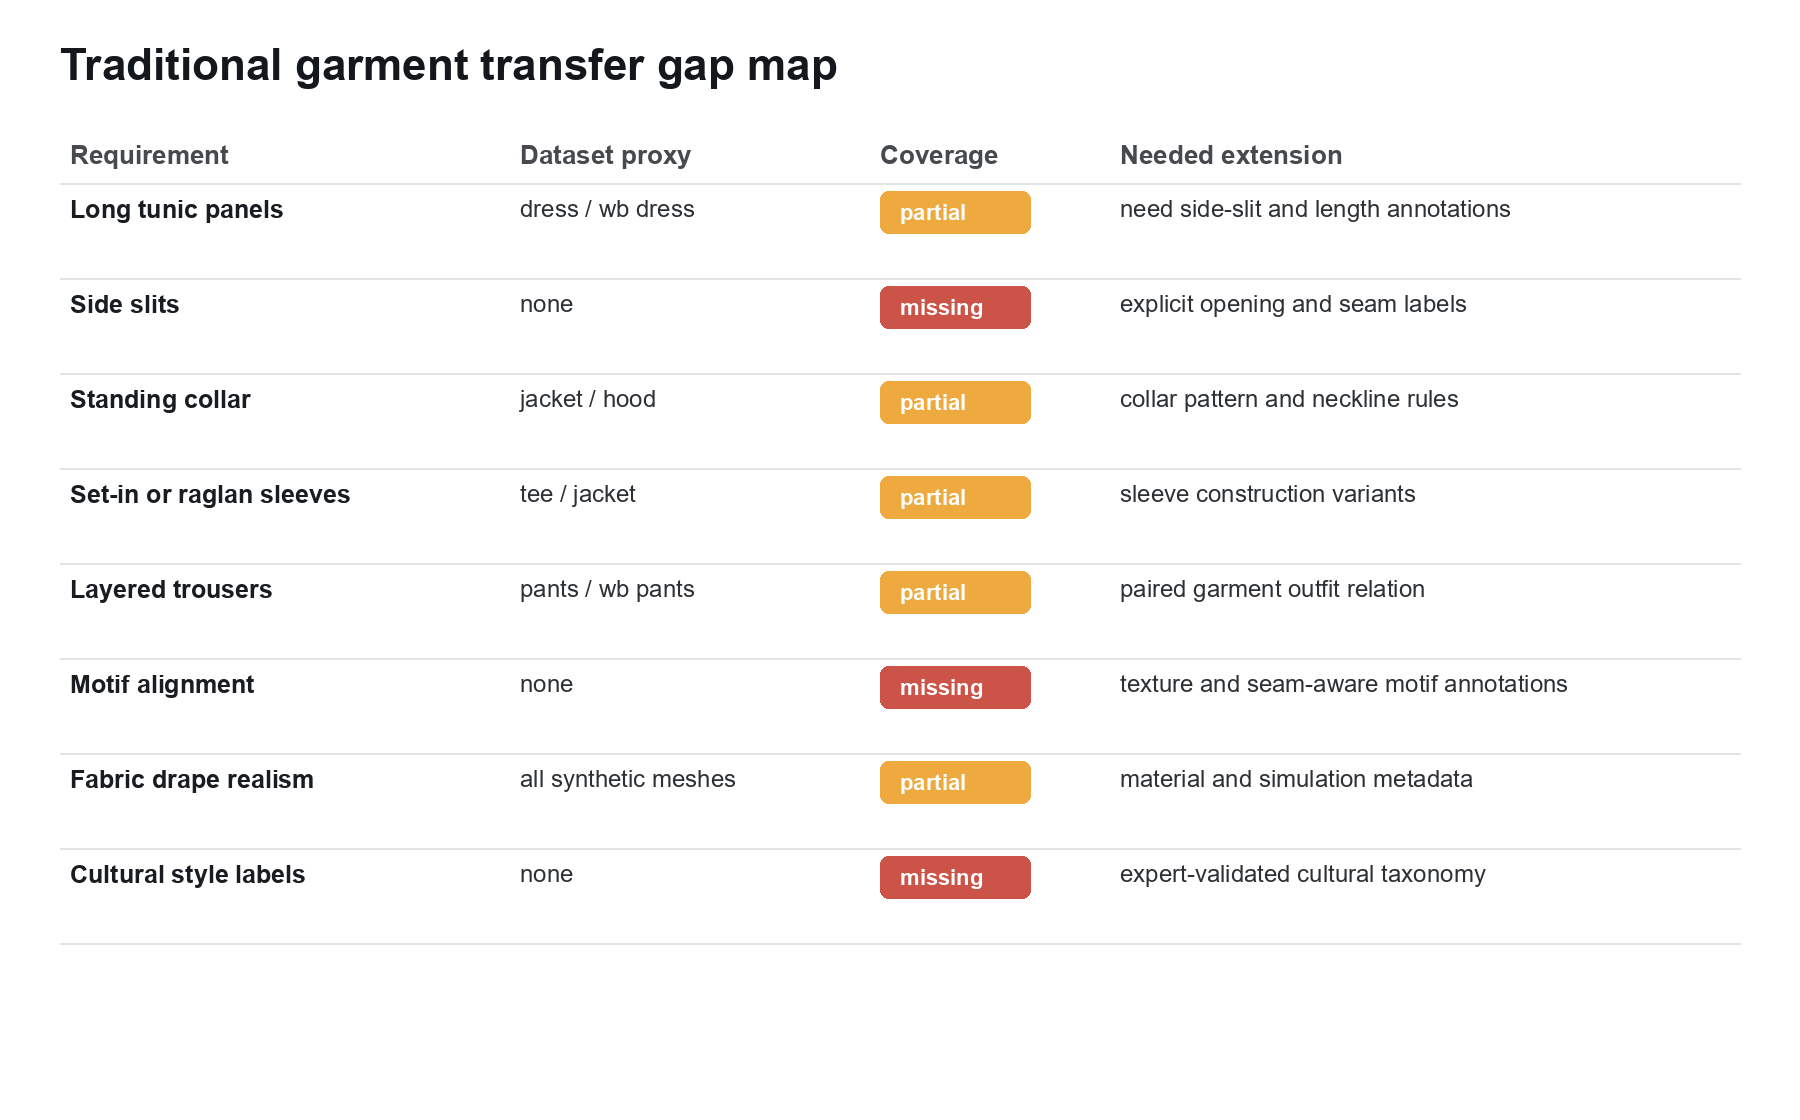
\includegraphics[width=\textwidth]{figures/fig_traditional_gap_map.png}
\caption{Traditional-garment transfer gap map. Existing structured garment categories provide useful proxies for some geometry and pattern components, but several culturally important requirements remain missing.}
\label{fig:traditionalgap}
\end{figure}

Nevertheless, the benchmark provides a concrete protocol for building such a dataset. A traditional-garment extension should collect or generate the same evidence tuple $(I,P,S,M,A)$, verify file-level completeness, compute mesh and pattern-graph descriptors, and report retrieval or reconstruction baselines before introducing a new neural model. This sequence would make the cultural extension auditable in the same way as the current full-data corpus. In this sense, the present work is a foundation study for traditional costume modeling rather than a direct solution to it.

\subsection{Limitations}

This paper does not train a deep reconstruction network and does not claim state-of-the-art image-to-pattern generation. The nearest-neighbor baselines are intentionally transparent and feature-based; they establish lower-cost reference points rather than replacing learned models. The benchmark does not yet evaluate Chamfer distance, normal consistency, IoU, physical simulation stability under predicted patterns, or texture/motif alignment. The dataset is synthetic and generated from template families, so results should not be interpreted as direct coverage of all real garments or traditional costume forms. Finally, pattern-only and combined baselines are very strong because structured pattern descriptors encode category-level template identity; future work should therefore separate input modalities carefully and report image-only or mesh-only settings when claiming reconstruction ability from weak evidence.

\subsection{Reproducibility and Extended Diagnostics}\label{sec:reproducibility}

\subsubsection{Benchmark Split Details}\label{sec:splits}

Table~\ref{tab:splits} gives the exact stratified split used by the retrieval and reconstruction baselines. The split is deterministic with a fixed random seed and preserves the category distribution of the full 22,450-sample production subset. Reporting the split explicitly is important because small category shifts can change nearest-neighbor retrieval difficulty. The table also makes later comparisons easier, since future learned models can reuse the same train, validation, and test counts.

\begin{table}[!htbp]
\caption{Deterministic 70/15/15 category-stratified split used for retrieval and reconstruction baselines.}\label{tab:splits}
\centering
\footnotesize
\begin{tabular}{lrrrr}
\toprule
Category & Train & Validation & Test & Total \\
\midrule
Dress sleeveless & 1,785 & 382 & 383 & 2,550 \\
Jacket & 1,540 & 330 & 330 & 2,200 \\
Jacket hood & 1,890 & 405 & 405 & 2,700 \\
Jumpsuit sleeveless & 1,400 & 300 & 300 & 2,000 \\
Pants straight sides & 700 & 150 & 150 & 1,000 \\
Skirt 2 panels & 840 & 180 & 180 & 1,200 \\
Skirt 4 panels & 1,120 & 240 & 240 & 1,600 \\
Skirt 8 panels & 700 & 150 & 150 & 1,000 \\
Tee & 1,610 & 345 & 345 & 2,300 \\
Tee sleeveless & 1,260 & 270 & 270 & 1,800 \\
WB dress sleeveless & 1,820 & 390 & 390 & 2,600 \\
WB pants straight & 1,050 & 225 & 225 & 1,500 \\
\midrule
Total & 15,715 & 3,367 & 3,368 & 22,450 \\
\bottomrule
\end{tabular}
\end{table}

\subsubsection{Per-Category Retrieval Diagnostics}\label{sec:percat}

Table~\ref{tab:percategory} reports category-level top-1 retrieval accuracy for mesh-only, segmentation-only, and combined nearest-neighbor baselines. Mesh-only retrieval is strong for pants and waistband variants but substantially weaker for jackets, hooded jackets, tees, and sleeveless tees, where geometry statistics alone confuse related upper-body garments. Segmentation features improve jacket and hooded-jacket separation but are weaker on some skirt and dress variants. The combined feature set is nearly perfect, with a single observed category error in the tee category.

\begin{table}[!htbp]
\caption{Per-category top-1 retrieval accuracy for feature-based nearest-neighbor baselines.}\label{tab:percategory}
\centering
\footnotesize
\setlength{\tabcolsep}{4pt}
\begin{tabular*}{\textwidth}{@{\extracolsep{\fill}}lrrrr}
\toprule
Category & Test \(N\) & Mesh & Segmentation & Combined \\
\midrule
Dress sleeveless & 383 & 0.935 & 0.794 & 1.000 \\
Jacket & 330 & 0.500 & 1.000 & 1.000 \\
Jacket hood & 405 & 0.511 & 0.983 & 1.000 \\
Jumpsuit sleeveless & 300 & 0.937 & 1.000 & 1.000 \\
Pants straight sides & 150 & 1.000 & 1.000 & 1.000 \\
Skirt 2 panels & 180 & 0.867 & 0.794 & 1.000 \\
Skirt 4 panels & 240 & 0.871 & 0.692 & 1.000 \\
Skirt 8 panels & 150 & 0.800 & 0.933 & 1.000 \\
Tee & 345 & 0.588 & 0.843 & 0.997 \\
Tee sleeveless & 270 & 0.596 & 0.804 & 1.000 \\
WB dress sleeveless & 390 & 0.951 & 0.823 & 1.000 \\
WB pants straight & 225 & 0.991 & 0.924 & 1.000 \\
\bottomrule
\end{tabular*}
\end{table}

\subsubsection{Ablation Matrix and Error Counts}\label{sec:ablation}

Table~\ref{tab:ablationmatrix} consolidates all retrieval settings into a single ablation ladder. The ordering is informative. Mesh statistics are useful but remain a relatively weak proxy for sewing-pattern identity. Segmentation labels are closer to pattern structure and improve both category retrieval and count prediction. Render descriptors are much stronger in this controlled corpus, but the error gallery in Fig.~\ref{fig:rendererrors} shows that the remaining mistakes occur between visually similar families. Pattern and combined structured features form an upper-bound setting rather than a realistic weak-input setting, because they expose the target construction evidence directly.

\begin{table}[!htbp]
\caption{Full modality ablation matrix for the retrieval-style reconstruction benchmark.}
\label{tab:ablationmatrix}
\centering
\footnotesize
\begin{tabular}{lrrrrr}
\toprule
Input modality & Features & Top-1 & Top-5 & MRR & Count MAE \\
\midrule
Random category & 0 & 0.0814 & 0.4167 & 0.0000 & 0.000/0.000 \\
Majority category & 0 & 0.1202 & 0.5502 & 0.0000 & 0.000/0.000 \\
Mesh statistics & 14 & 0.7732 & 0.9543 & 0.8504 & 0.664/1.426 \\
Segmentation statistics & 8 & 0.8812 & 0.9774 & 0.9235 & 0.005/0.101 \\
Front render & 375 & 0.9973 & 0.9997 & 0.9985 & 0.006/0.009 \\
Back render & 375 & 0.9973 & 0.9994 & 0.9983 & 0.006/0.010 \\
Front/back render & 1,125 & 0.9970 & 0.9997 & 0.9983 & 0.005/0.011 \\
Pattern descriptors & 9 & 1.0000 & 1.0000 & 1.0000 & 0.000/0.000 \\
Pattern+mesh+segmentation & 31 & 0.9997 & 0.9997 & 0.9997 & 0.001/0.002 \\
\bottomrule
\end{tabular}
\end{table}

The paired render descriptor produces only ten top-1 errors over 3,368 test samples. Table~\ref{tab:rendererrorsummary} groups those errors by source and retrieved category. The table supports the visual diagnosis in Fig.~\ref{fig:rendererrors}: most failures are between neighboring garment families, especially jacket--tee and pants--waistband-pants. The result is useful for future model papers because it gives a compact checklist of the cases that a learned image-to-pattern method should improve beyond simple deterministic retrieval.

\begin{table}[!htbp]
\caption{Top-1 error summary for paired front/back render retrieval.}
\label{tab:rendererrorsummary}
\centering
\footnotesize
\begin{tabular}{lrr}
\toprule
Confusion pair & Errors & Interpretation \\
\midrule
Jacket $\rightarrow$ tee & 2 & Similar upper-body silhouette at descriptor scale \\
Tee $\rightarrow$ jacket & 2 & Sleeve and torso cues dominate closure details \\
Tee $\rightarrow$ sleeveless tee & 1 & Sleeve evidence is weak after resizing \\
Pants $\rightarrow$ waistband pants & 1 & Waistband cue is visually subtle \\
Waistband pants $\rightarrow$ pants & 2 & Lower-body geometry dominates waistband detail \\
Waistband dress $\rightarrow$ jumpsuit & 1 & Full-body silhouette ambiguity \\
Eight-panel skirt $\rightarrow$ pants & 1 & Lower-body shape is underrepresented in thumbnail features \\
\bottomrule
\end{tabular}
\end{table}

\subsubsection{Retrieval Confusion Matrices}\label{sec:confusion}

The confusion matrices in Fig.~\ref{fig:confusionpanel} diagnose where the feature families fail. Mesh-only retrieval produces meaningful off-diagonal structure: jackets and hooded jackets are often confused with each other, tees and sleeveless tees are confused with related upper-body garments, and skirt categories occasionally shift along the skirt complexity ladder. Segmentation features reduce jacket/hood confusion because panel labels encode stronger structural evidence. Combined features nearly diagonalize the confusion matrix. The paired render descriptor is also nearly diagonal, confirming that controlled rendered appearance is a very strong category cue in this corpus. The pattern-only confusion matrix is retained as an experiment artifact but omitted from the paper layout because Table~\ref{tab:ablationmatrix} already reports the perfect pattern-descriptor upper bound.

\begin{figure}[!htbp]
\centering
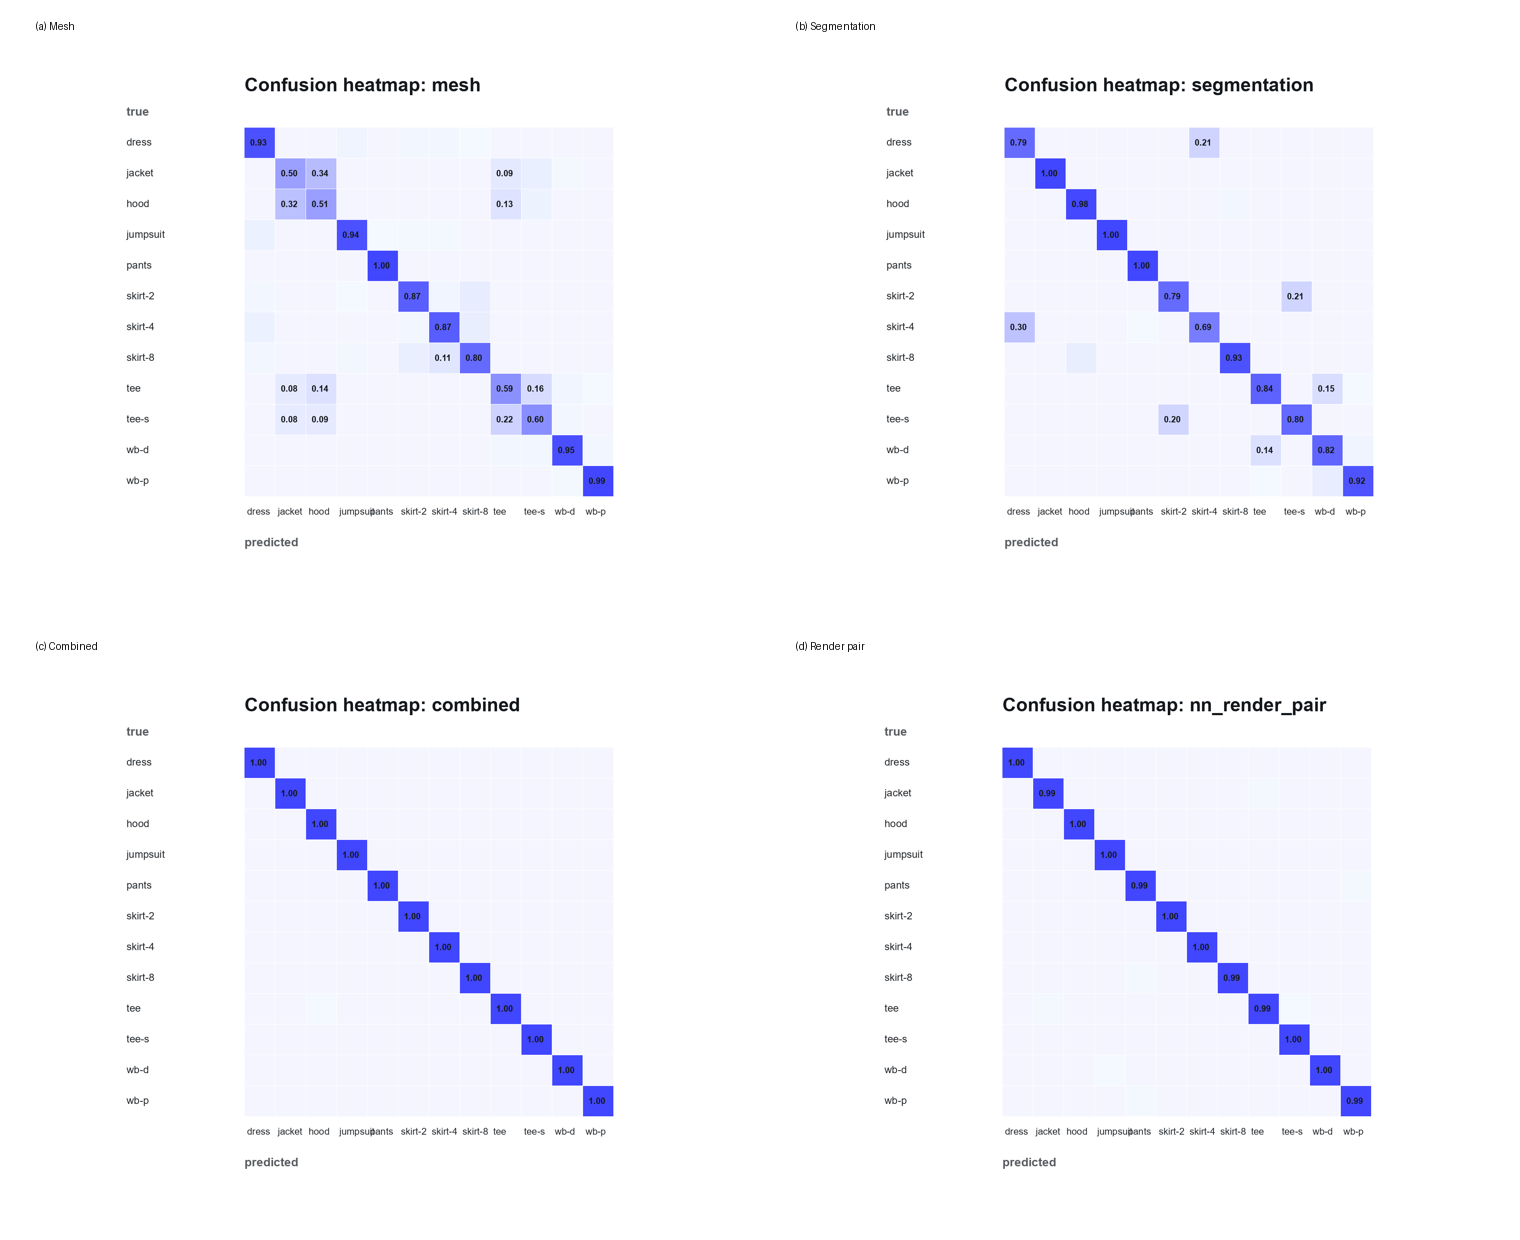
\includegraphics[width=\textwidth,height=0.86\textheight,keepaspectratio]{figures/fig_confusion_matrix_panel.png}
\caption{Row-normalized confusion matrices for four retrieval settings: (a) mesh-only, (b) segmentation-only, (c) combined pattern, mesh, and segmentation, and (d) paired front/back render descriptors.}
\label{fig:confusionpanel}
\end{figure}

\subsubsection{Metric Definitions and Reproducibility Notes}\label{sec:metrics}

The benchmark outputs one measurement row per production sample and keeps the following metric groups. Evidence metrics record the presence of front and back renders, raster and vector pattern evidence, simulated and scan-imitation meshes, mesh segmentations, and garment specifications. Pattern metrics record panel count, pattern-edge count, stitch count, graph components, mean panel area, total panel area, mean panel perimeter, curved-edge count, and parameter count. Mesh metrics are computed separately for simulated and scan-imitation meshes and include vertices, faces, used and unused vertices, unique edges, boundary edges, non-manifold edges, connected components, duplicate vertices, degenerate faces, edge-length statistics, triangle-area statistics, and aspect-ratio statistics. Segmentation metrics include total segmentation lines, label count, non-stitch panel-label count, stitch-label fraction, and label entropy.

All heavy metrics are computed by streaming archive members directly from the verified compressed files. The benchmark does not require full extraction of the 84.77 GB compressed corpus. Intermediate per-archive measurements are written immediately after each archive finishes, which makes the experiment auditable and partially resumable. The full quantitative pass parses 22,450 production samples and produces the merged benchmark table, category summary, consistency histogram, mesh-quality figure, pattern-structure figure, skirt-complexity ladder, retrieval baseline table, split definitions, confusion matrices, and experiment reports.

The render-image baseline uses deterministic descriptors rather than learned visual embeddings. This choice keeps the baseline reproducible without GPU training and exposes how much category information is already available from controlled render appearance. Each view descriptor contains a low-resolution grayscale thumbnail, edge-filter responses, RGB histograms, channel means, channel standard deviations, and a binary view-presence indicator. The paired descriptor concatenates front, back, and absolute front-back difference descriptors. This baseline should be interpreted as an in-distribution render retrieval test, not as a claim that real photographs can be reconstructed at the same accuracy.

\subsubsection{Artifact Inventory}\label{sec:artifacts}

Table~\ref{tab:artifacts} summarizes the concrete artifacts produced by the benchmark. The separation into experiment directories is intentional: the initial evidence audit, quantitative mesh-pattern benchmark, structured-feature retrieval, render-image retrieval, and manuscript-specific diagnostic figures can be rerun or inspected independently. This inventory also clarifies which outputs are raw measurements and which outputs are manuscript-level summaries. It therefore helps readers reproduce the paper without treating the PDF figures as the only available evidence.

\begin{table}[!htbp]
\caption{Experiment artifact inventory.}\label{tab:artifacts}
\centering
\footnotesize
\begin{tabular}{p{0.24\textwidth}p{0.66\textwidth}}
\toprule
Experiment & Main artifacts \\
\midrule
Evidence audit & File manifest, checksum status, full sample evidence table, per-category audit tables, missing-evidence report, category summary, render-pattern evidence sheet, and category complexity figure. \\
Quantitative benchmark & Full production benchmark table with pattern, mesh, segmentation, and consistency metrics; per-category quantitative summary; mesh-quality figure; pattern-structure figure; consistency histogram; skirt complexity ladder. \\
Structured retrieval & Deterministic train/validation/test split, structured-feature nearest-neighbor baselines, per-category top-1 tables, confusion matrices, retrieval benchmark report. \\
Render retrieval & Cached render-image feature matrix, render feature metadata, front/back/pair render retrieval baselines, render confusion matrix, qualitative retrieval examples, render error gallery. \\
Extra manuscript figures & Code-generated render error gallery and traditional-garment transfer gap map used by the manuscript. \\
\bottomrule
\end{tabular}
\end{table}

\subsubsection{Evaluation Protocol Card}\label{sec:protocol}

The benchmark is intended to separate evidence quality from model ability. Table~\ref{tab:protocolcard} states the recommended interpretation of each metric group. This distinction matters because several metrics are necessary preconditions for reconstruction, not final reconstruction scores. The protocol card prevents a common error in garment reconstruction papers: treating high category retrieval accuracy as if it were already evidence of accurate sewing-pattern reconstruction.

\begin{table}[!htbp]
\caption{Recommended interpretation of benchmark metric groups.}\label{tab:protocolcard}
\centering
\footnotesize
\begin{tabular}{p{0.22\textwidth}p{0.34\textwidth}p{0.34\textwidth}}
\toprule
Metric group & What it proves & What it does not prove \\
\midrule
Evidence completeness & Required files exist and can be located reproducibly. & Geometry, pattern correctness, or simulation quality. \\
Pattern graph metrics & Panel, edge, stitch, and graph complexity are extractable from specifications. & That a model can infer those structures from images. \\
Mesh quality metrics & Meshes are parseable and have measurable geometric regularity. & Physical validity under new body poses or materials. \\
Segmentation metrics & Mesh vertices can be related to panel-like labels. & Semantic correctness of every boundary or seam. \\
Consistency score & Pattern, mesh, and segmentation evidence are jointly usable for benchmark construction. & Chamfer distance, normal consistency, or final reconstruction accuracy. \\
Retrieval baselines & Simple nearest-neighbor methods provide transparent lower-cost references. & Learned generalization to unseen templates, colors, bodies, or real photographs. \\
Render baseline & Controlled rendered views contain strong category and template cues. & Real-world photo-to-pattern reconstruction performance. \\
\bottomrule
\end{tabular}
\end{table}

For future learned models, we recommend reporting at least four settings: image-only, mesh-only, segmentation-assisted, and pattern-assisted. Image-only experiments should include the deterministic render baseline. Mesh-only experiments should compare against the mesh nearest-neighbor baseline. Segmentation-assisted experiments should state whether segmentation is ground truth or predicted. Pattern-assisted experiments should be treated as upper-bound or retrieval settings unless the pattern input is intentionally part of the task.

\subsubsection{Traditional-Garment Dataset Schema}\label{sec:traditionalschema}

Table~\ref{tab:traditionalschema} gives a minimum schema for extending the benchmark toward traditional garments. The schema is phrased generically, but it is motivated by garments such as the Vietnamese \textit{ao dai}, where silhouette, side openings, collar construction, trouser pairing, and motif placement are culturally meaningful rather than cosmetic metadata. The goal is to define what must be measured before a reconstruction model is trained. Without such fields, a dataset may support visual similarity while still missing construction and cultural validity.

\begin{table}[!htbp]
\caption{Minimum schema for a traditional-garment pattern-reconstruction dataset.}\label{tab:traditionalschema}
\centering
\footnotesize
\begin{tabular}{p{0.24\textwidth}p{0.66\textwidth}}
\toprule
Field group & Required content \\
\midrule
Visual evidence & Front, back, side, and detail views under controlled lighting; optional real-photo views if available; explicit camera metadata. \\
Pattern evidence & Editable 2D panels, panel names, edge loops, seam allowances, darts, pleats, slits, collar pieces, sleeve variants, and trouser components. \\
Stitch evidence & Stitch pairs, seam type, open-boundary labels, side-slit labels, collar attachment, sleeve attachment, and layered-garment relations. \\
Mesh evidence & Simulated garment mesh, scan or scan-imitation mesh, vertex-to-panel segmentation, boundary-edge labels, and body-fit metadata. \\
Material evidence & Fabric type, stiffness or drape class, transparency, lining, and simulation parameters when available. \\
Motif evidence & Texture image, motif class, motif placement rules, seam-crossing continuity, and alignment constraints across panels. \\
Cultural metadata & Garment subtype, region or community label if ethically appropriate, time period, usage context, and expert validation status. \\
Evaluation splits & Category-stratified and style-stratified splits, plus cross-style or cross-region splits for generalization claims. \\
\bottomrule
\end{tabular}
\end{table}

\begin{figure}[!htbp]
\centering
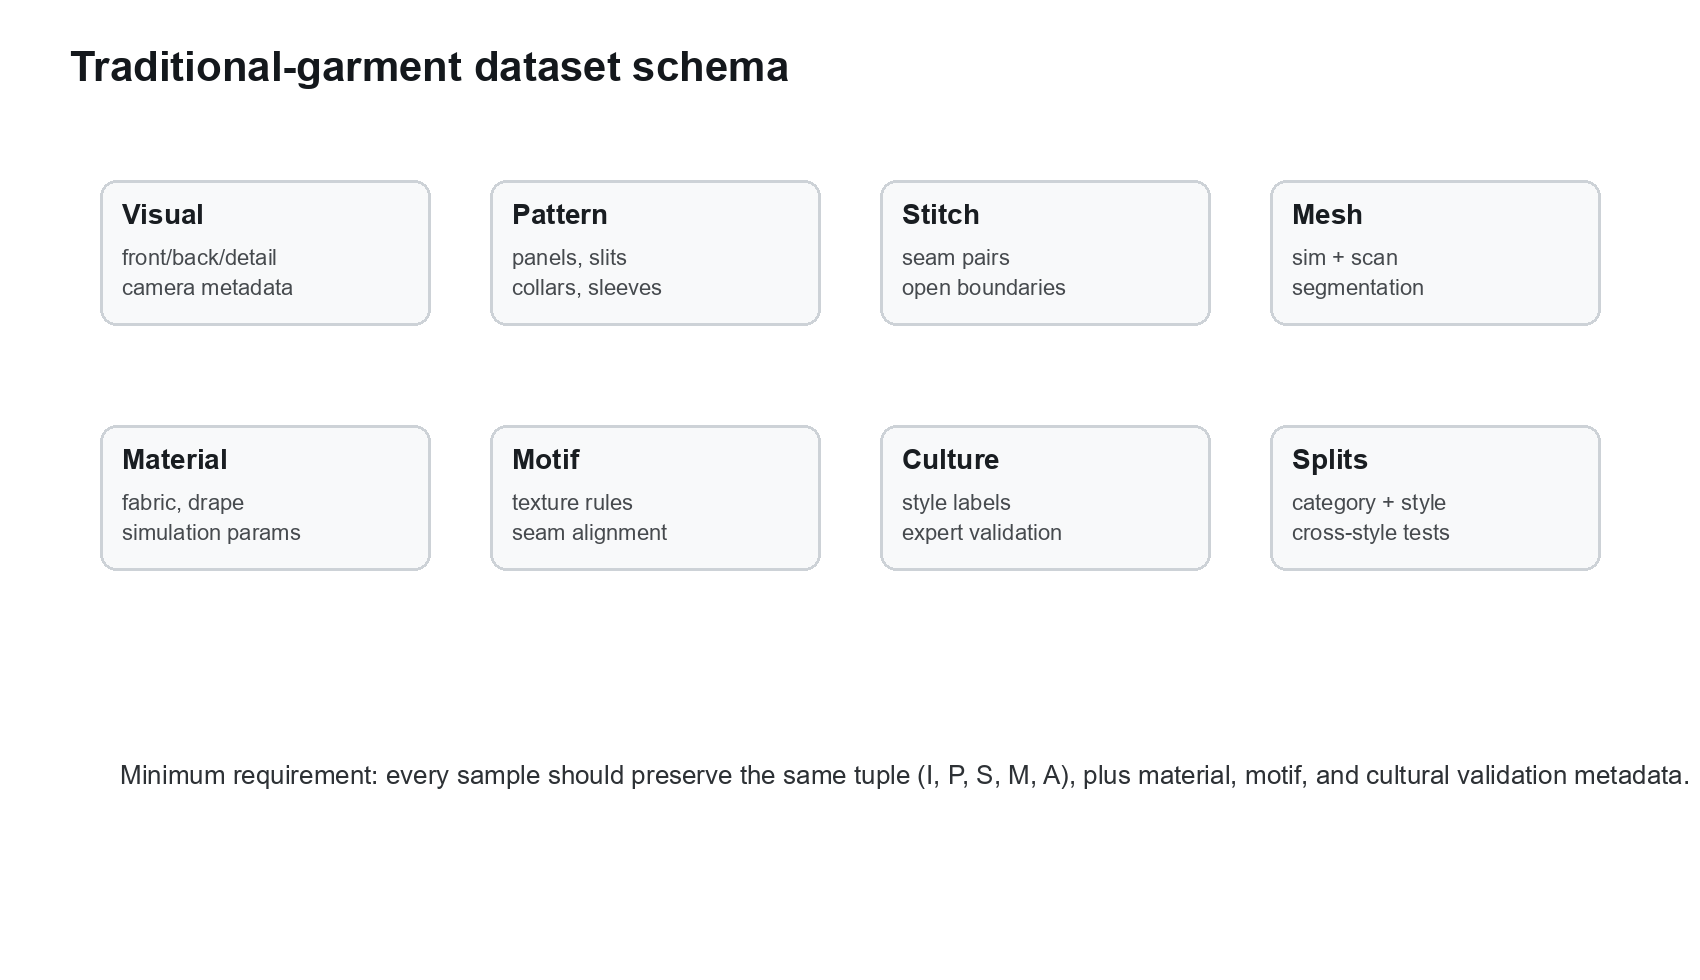
\includegraphics[width=0.95\textwidth]{figures/fig_traditional_schema_flow.png}
\caption{Minimum evidence schema for extending the benchmark toward traditional garments. The schema preserves the core render-pattern-stitch-mesh-attribute tuple and adds material, motif, cultural validation, and cross-style split metadata.}
\label{fig:traditionalschema}
\end{figure}

This schema is intentionally stricter than what is needed for generic garment retrieval. Traditional costume modeling risks producing visually plausible but culturally incorrect assets if side slits, collars, layered trousers, textile motifs, and expert labels are absent. The additional fields also support more meaningful generalization tests, such as cross-style, cross-region, or motif-transfer splits. The current benchmark therefore supplies the measurement protocol, while a traditional-garment corpus must supply the missing cultural and construction evidence.

\section{Conclusion}\label{sec:conclusion}

This study presents a full-data sewing-pattern reconstruction benchmark on 22,457 structured garment samples, including a 22,450-sample production subset. The corpus was downloaded, checksum-verified, audited directly from archive files, and parsed for pattern, mesh, segmentation, and consistency metrics. The results show 99.98\% complete evidence, 99.996 mean pattern-mesh consistency in the production subset, and a broad structural ladder from two-panel skirts to nine-panel hooded jackets. Retrieval baselines show that mesh and segmentation evidence provide nontrivial but imperfect proxies for pattern structure, while combined structured features nearly recover category and panel/stitch structure in distribution. The hard-generalization results add an important caution: high render retrieval on the random split mainly reflects controlled-view and template regularity, so stronger claims require held-template or domain-shift protocols. The resulting audit tables, benchmark metrics, splits, baselines, and code-generated figures provide a concrete foundation for later learned pattern-reconstruction and pattern-generation models on verified full-data garment assets.

\backmatter

\section*{Data availability}
The audited dataset is available from the Zenodo record for the Dataset of 3D Garments with Sewing Patterns: \url{https://zenodo.org/records/5267549}. The code, experiment outputs, benchmark summaries, generated figures, and manuscript source are available at \url{https://github.com/ictu-se/sewing-pattern-reconstruction-benchmark}.

\bibliography{references}

\end{document}
